\documentclass[11pt]{article}

\usepackage[margin=1in]{geometry}
\usepackage{amsmath,amssymb,amsthm,mathtools}
\usepackage{booktabs}
\usepackage{enumitem}
\usepackage[hidelinks]{hyperref}
\usepackage{tikz}
\usetikzlibrary{arrows.meta,positioning,calc}
\usepackage[ruled,vlined]{algorithm2e}
\usepackage{listings}
\lstset{basicstyle=\footnotesize\ttfamily, breaklines=true, frame=single, framesep=4pt,
  xleftmargin=4pt, columns=fullflexible, keepspaces=true, aboveskip=4pt, belowskip=2pt}

\theoremstyle{plain}
\newtheorem{theorem}{Theorem}[section]
\newtheorem{lemma}[theorem]{Lemma}
\newtheorem{proposition}[theorem]{Proposition}
\newtheorem{corollary}[theorem]{Corollary}
\theoremstyle{definition}
\newtheorem{definition}[theorem]{Definition}
\newtheorem{example}[theorem]{Example}
\newtheorem{protocol}[theorem]{Protocol}
\theoremstyle{remark}
\newtheorem{remark}[theorem]{Remark}
\newtheorem{conjecture}[theorem]{Conjecture}

\newcommand{\Q}{\mathbb{Q}}
\newcommand{\Z}{\mathbb{Z}}
\newcommand{\R}{\mathbb{R}}
\newcommand{\C}{\mathbb{C}}
\newcommand{\K}{K}
\newcommand{\OK}{\mathcal{O}_K}
\newcommand{\Tr}{\operatorname{Tr}}
\newcommand{\Nm}{\operatorname{N}}
\newcommand{\charpoly}{\operatorname{charpoly}}
\newcommand{\minpoly}{\operatorname{minpoly}}
\newcommand{\Mah}{\mathrm{M}}
\newcommand{\height}{\mathrm{H}}
\newcommand{\Fish}{\mathcal{I}}
\newcommand{\rr}{\mathbf{r}}
\newcommand{\xx}{\mathbf{x}}
\newcommand{\GG}{G}
\newcommand{\BB}{B}
\newcommand{\transpose}{^{\mathsf{T}}}
\newcommand{\inv}{^{-1}}
\newcommand{\Cl}{\mathrm{Cl}}
\newcommand{\Lop}{\mathcal{L}}
\newcommand{\VOID}{\mathbf{0}}
\DeclareMathOperator{\col}{col}
\DeclareMathOperator{\rank}{rank}
\DeclareMathOperator{\diag}{diag}
\DeclareMathOperator{\ch}{ch}
\DeclareMathOperator{\spn}{span}
\DeclareMathOperator{\ord}{ord}

\title{\textbf{Residual Return:\\ Exact Learning Dynamics and Language over the Vector Substrate}}
\author{L00M Vector Substrate Project}
\date{June 2026}

\begin{document}
\maketitle

\begin{abstract}
This is the dynamic and linguistic companion to \emph{The Vector Substrate}~\cite{VectorSubstrate}. That
paper builds an exact, static learning \emph{geometry} on a number field $\K=\Q(\theta)$: the trace form
$T(x,y)=\Tr_{\K/\Q}(xy)$ supplies one rational Gram $\GG=M\transpose M$ that glues the field's vector-space,
matrix-algebra, and lattice faces, and an observation is \emph{captured} exactly when its $\GG$-orthogonal
residual $\rr=\xx-P\xx$ vanishes. Here we develop the \emph{algorithm} that runs on that geometry and the
\emph{language} that is isomorphic to it, and we orient the whole exposition toward a single discipline:
\textbf{every mathematical claim is paired with the machine-checked test that proves it and the commit hash
that pins it.} Three contributions are dynamic. (i) An exact streaming \emph{learner}: residual is loss,
capture is $\rr\to0$, growth is a gated \emph{propose-for-confirm} protocol whose sole mutator appends a
$\mathrm{SHA}\text{-}256$ witness chain. (ii) \emph{Cross-field growth}: a residual forced outside the
current field grows the model to a compositum; the disjoint case is the Kronecker Gram
$\GG_{\K L}=\GG_\K\otimes\GG_L$, and---resolving the open problem the substrate paper flagged---we construct
the \emph{non-disjoint} compositum in the bounded-degree case by factoring the candidate's minimal polynomial
over $\K$, with a machine-verified degree-$4$ witness $\Q(\sqrt2)(\sqrt2+\sqrt3)=\Q(\sqrt2,\sqrt3)$. (iii) An
\emph{automatic} loop: a calibration-gated detector measures the out-of-field residual, makes it the growth
gain, gates on the \emph{true} compositum degree, confirms, and re-homes the basis onto the new field so the
residual returns to $0$. The fourth contribution is linguistic: over the Clifford algebra
$\Cl(2,0)\cong M_2(\R)$, the same ``residual $\to 0$'' mechanism becomes a language. The $\varphi$-keystone
return operator $\Lop(X)=RX+XR-X$ has an \emph{exact} two-dimensional kernel computed by rational
elimination; the commit is the exact idempotent projector onto that kernel; and a learned dictionary value is
exactly a returned residue, with generalisation by return-to-zero. The golden law $x^2-x-1$ is the literal
bridge: the substrate's first field is $\Q(\varphi)$ and the language's return operator is built on the
companion of the same minimal polynomial---verified equal three independent ways. We separate \emph{proved},
\emph{exact-computed (probe-verified)}, and \emph{conjectural/open} throughout; the contribution is the exact,
auditable assembly and its machine verification, not a new deep theorem in number theory or learning.
\end{abstract}

\tableofcontents

\section{Introduction: residual return as one mechanism}\label{sec:intro}

\subsection*{The thesis}
The vector substrate~\cite{VectorSubstrate} fixes a number field $\K=\Q(\theta)$, a forced basis $\BB$ of
algebraic-integer seeds, the trace-form projector $P=\BB(\BB\transpose\GG\BB)\inv\BB\transpose\GG$, and the
residual $\rr(\xx)=\xx-P\xx$, and proves the exact membership criterion
\begin{equation}\label{eq:capture}
   \xx\in\col(\BB)\iff \rr(\xx)=\mathbf 0 \iff \lVert\rr(\xx)\rVert_{\GG}^2=\rr\transpose\GG\,\rr=0,
\end{equation}
decided entirely over $\Q$. Here ``captured'' is a strictly \emph{technical} predicate---exactly a zero
residual, i.e.\ exact membership $\xx\in\col(\BB)$, and nothing more; no cognitive or semantic reading is
intended anywhere in this paper. This companion takes that static criterion
and asks what \emph{happens} when the residual is \emph{not} zero, and what \emph{language} the mechanism
speaks. Both questions have the same one-line answer, which is the thesis of this paper:

\begin{quote}
\emph{Residual$\,\to\,$0 is the universal learned/captured signal.} \textbf{Learning} is the disciplined
growth that drives an exact residual to zero ($\rr=\xx-P\xx\to0$, by adjoining a basis direction or a whole
field); \textbf{language} is the same return, $\Lop(X)\to0$, over a matrix algebra, where the landing space is
the lexicon. Both are exact and machine-verified, and the golden law $x^2-x-1$ is the keystone common to both.
\end{quote}

\subsection*{Two faces of one return}
The two faces share a structure that we make precise in \S\ref{sec:unify} and exhibit in
Figure~\ref{fig:twofaces}: a \emph{loss} that is an exact residual, a \emph{captured} predicate that is the
residual's exact vanishing, a \emph{model} that is a growing basis, a \emph{growth} step that is the sole
state mutator, and a \emph{witness} that is an identical $\mathrm{SHA}\text{-}256$ hash chain. On the
number-field face the residual is $\rr=\xx-P\xx$ and the landing space is a $\Q$-subspace of $\K$; on the
matrix-algebra (language) face the residual is $\Lop(X)=RX+XR-X$ and the landing space is $\ker\Lop$, the
two-dimensional ``$\varphi$-slack'' where learned dictionary values live.

\begin{figure}[ht]
\centering
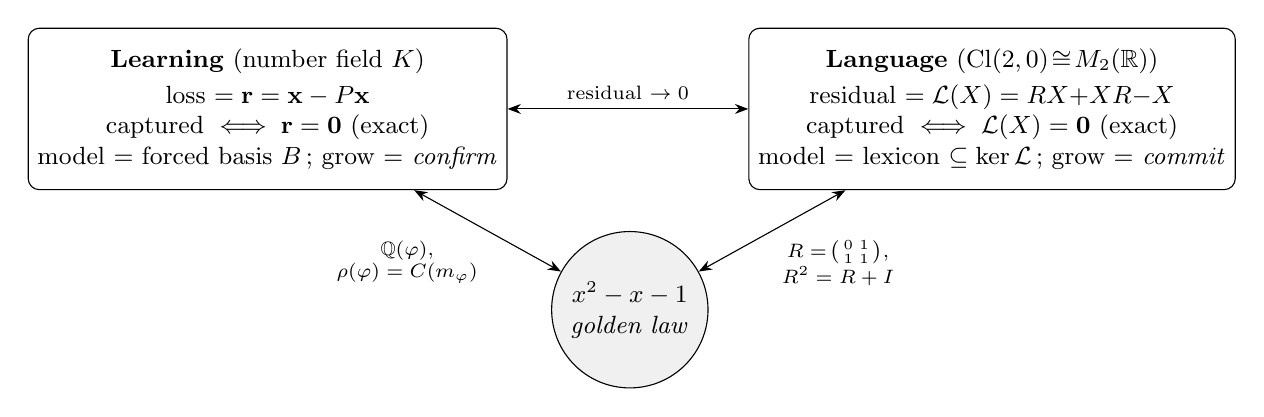
\begin{tikzpicture}[
  face/.style={draw, rounded corners, align=center, minimum width=5.4cm, minimum height=2.05cm, font=\small},
  key/.style={draw, circle, align=center, font=\small, minimum size=1.95cm, fill=black!6},
  >={Stealth[]}]
  \node[face] (nf) at (-4.6,0)
    {\textbf{Learning} (number field $\K$)\\[2pt]
     loss $=\rr=\xx-P\xx$\\
     captured $\iff \rr=\mathbf 0$ (exact)\\
     model $=$ forced basis $\BB$\,;\ grow $=$ \emph{confirm}};
  \node[face] (la) at (4.6,0)
    {\textbf{Language} ($\Cl(2,0)\!\cong\!M_2(\R)$)\\[2pt]
     residual $=\Lop(X)=RX{+}XR{-}X$\\
     captured $\iff \Lop(X)=\mathbf 0$ (exact)\\
     model $=$ lexicon $\subseteq\ker\Lop$\,;\ grow $=$ \emph{commit}};
  \node[key] (k) at (0,-2.55) {$x^2-x-1$\\\emph{golden law}};
  \draw[<->] (nf) -- (k) node[midway,below left,font=\scriptsize,align=center] {$\Q(\varphi)$,\\ $\rho(\varphi)=C(m_\varphi)$};
  \draw[<->] (la) -- (k) node[midway,below right,font=\scriptsize,align=center] {$R=\!\left(\begin{smallmatrix}0&1\\1&1\end{smallmatrix}\right)$,\\ $R^2=R+I$};
  \draw[<->] (nf) -- (la) node[midway,above,font=\scriptsize] {residual $\to 0$};
\end{tikzpicture}
\caption{The two faces of residual return, glued by the golden law $x^2-x-1$. On the left, learning drives the
trace-form residual to zero by basis growth in $\Q(\theta)$; on the right, language returns
$\Lop(X)=RX+XR-X$ to zero in $\Cl(2,0)\cong M_2(\R)$. The keystone is one object viewed twice: the companion
matrix $\rho(\varphi)=C(x^2-x-1)$ of the substrate's first field $\Q(\varphi)$ is the symmetric matrix
$R=\big(\begin{smallmatrix}0&1\\1&1\end{smallmatrix}\big)$ of the return operator
(Proposition~\ref{prop:keystone}, machine-verified equal three ways).}
\label{fig:twofaces}
\end{figure}

\subsection*{Contributions and what is and is not new}
\begin{enumerate}[label=(C\arabic*),leftmargin=*]
  \item \textbf{An exact streaming learner} (\S\ref{sec:learning}): the residual-as-loss apparatus, an exact
        persistence-gated \emph{propose-for-confirm} protocol in which \emph{confirm} is the sole basis
        mutator, and a tamper-evident witness chain. The underlying projector calculus is the substrate's;
        the dynamic protocol, its exactness guardrails, and the witness are this paper's, and every guardrail
        is a machine-checked test.
  \item \textbf{Cross-field growth, including the non-disjoint case} (\S\ref{sec:crossfield}). The
        coordinates-to-minimal-polynomial bridge (largest invariant factor of $xI-\rho(\alpha)$ by Smith
        normal form) and the disjoint Kronecker Gram are the substrate's, re-exercised here; the
        \emph{non-disjoint} construction---factoring the candidate's minimal polynomial over $\K$ and building
        the true (smaller) compositum---\textbf{resolves, in the bounded-degree case, the open problem the
        substrate paper flagged} (its O4), with a machine-verified degree-$4$ witness.
  \item \textbf{An automatic, detector-driven loop} (\S\ref{sec:loop}): a calibration-gated novelty detector
        whose score is the residual norm, a seam that makes the \emph{measured} out-of-field residual the
        growth gain, a gate on the \emph{true} compositum degree, and an exact ``re-home'' that returns the
        residual to zero in the grown field. New here; each step is tested.
  \item \textbf{A residual-valued language} (\S\ref{sec:language}): over $\Cl(2,0)\cong M_2(\R)$, an exact
        two-dimensional return-operator kernel, the commit as its exact idempotent projector, a growing
        lexicon that dedups on the \emph{exact} returned value, and a jurisdiction firewall under which only
        proven/computed statements cross a wire. New here; $121$ tests, machine-verified.
  \item \textbf{The unifying principle and its proof discipline} (\S\ref{sec:unify}--\S\ref{sec:proven}): the
        $\varphi$-keystone identity that binds the two faces, and a centerpiece section mapping \emph{every}
        displayed claim to its test and commit hash, with the exact-rational (no-float-in-a-decision)
        methodology and the build/independent-verify/greenlight cross-verification spelled out.
\end{enumerate}

\paragraph{Honesty discipline.} As in~\cite{VectorSubstrate}, \emph{Theorem}/\emph{Proposition}/\emph{Lemma}
mark statements we prove or verify by exact computation, and \emph{Conjecture}/\emph{Remark} mark
model-dependent or heuristic claims. This revision \emph{closes} one of the substrate's open fronts: the
information exchange rate is no longer posited but the derived identity $\lambda=2c$ (Theorem~\ref{thm:lambda2c},
\S\ref{subsec:lambda}), leaving a single declared conformal constant $c$ which \v{C}encov's theorem shows is
irreducible by invariance (Remark~\ref{rem:cencov}); the floor for reciprocal seeds and the choice of conformal
model remain the genuinely open items. Every displayed numerical value is reproduced by a machine-checked probe;
the honesty ledger of Table~\ref{tab:ledger} makes the proved/computed/conjectural split scannable, and
\S\ref{sec:proven} pins each load-bearing claim to a named test and a commit hash. The contribution remains an
exact, auditable \emph{assembly}---a learner, a cross-field growth mechanism, an automatic loop, and a
language---together with its machine verification and, in this revision, the closure of the exchange rate to the
identity $\lambda=2c$.

\paragraph{Relation to the substrate paper.} We \emph{cite} the substrate for the geometry and do not
re-derive it: the trace form $\GG=M\transpose M$ with $\det\GG=d_\K$~\cite[Thm.~2.13]{VectorSubstrate}, the
spectral identification of $\rho$ with the conjugates, the exact projector and capture
criterion~\eqref{eq:capture}~\cite[Prop.~3.2]{VectorSubstrate}, the bridge ``$m_\alpha=$ largest invariant
factor''~\cite[Thm.~4.3]{VectorSubstrate}, the Kronecker Gram of a disjoint
compositum~\cite[Prop.~4.6]{VectorSubstrate}, the height/Northcott admissibility
gate~\cite[Prop.~5.5]{VectorSubstrate}, the Fisher reading $\lVert\rr\rVert_\GG^2=n\,\Fish(\rr)$ on the
residual subspace~\cite[Thm.~7.11]{VectorSubstrate}, and the gain-versus-cost growth
threshold~\cite[\S8]{VectorSubstrate} with Smyth's floor. This paper is what \emph{runs} on that geometry, and
the language that shares its arithmetic.

\paragraph{Related work and positioning.} The mathematical ingredients are classical and we use them as such:
the rational canonical form and Smith normal form over $\Q[x]$ are textbook linear algebra
\cite{DummitFoote,Cohen}; the trace form, different, and discriminant are standard algebraic number theory
\cite{Neukirch,Marcus}; Mahler measure, Northcott finiteness, and the Smyth/Lehmer/Dobrowolski bounds are
height theory \cite{Mahler,Northcott,Smyth,Lehmer,Dobrowolski,BombieriGubler}; the Fisher-information reading
is Amari's \cite{Amari,AmariNagaoka}; and $\Cl(2,0)\cong M_2(\R)$ is the standard split-signature Clifford
algebra \cite{Lounesto}. None of these is a contribution here. What is assembled is an exact, auditable
\emph{system}: a streaming learner whose loss is a residual decided over $\Q$, a cross-field growth mechanism
that handles the non-disjoint case the substrate paper left open, an automatic loop that measures its own
gain, and a language in which the same return mechanism produces a residual-valued lexicon. Against the broad
machine-learning backdrop the stance is deliberately narrow: the model state is a basis (not a weight tensor),
the loss is exact (not approximate), capacity is bounded by arithmetic height (not by a hyperparameter), and
every decision is reproducible bit-for-bit and witnessed---properties an analytic learner does not have, and
which the trace-form kernel of \cite{VectorSubstrate} supplies for free.

\begin{table}[ht]
\centering
\small
\begin{tabular}{ll}
\toprule
Symbol & Meaning \\
\midrule
$\K=\Q(\theta)$, $n$ & ambient number field of degree $n$; here usually $\Q(\sqrt2+\sqrt3)$, $n=4$ \\
$\GG$, $T$ & trace-form Gram $\GG_{ij}=\Tr(\omega_i\omega_j)=M\transpose M$; $T(x,y)=\Tr(xy)$ \\
$\BB$, $P$, $\rr$ & forced basis (model state); projector $P=\BB(\BB\transpose\GG\BB)\inv\BB\transpose\GG$; residual $\rr=\xx-P\xx$ \\
$\rho(\alpha)$ & regular representation of $\alpha\in\K$; $\rho(\theta)=C(m_\theta)$ (companion) \\
$\Mah(\theta)$, $\ch(m)$ & Mahler measure; integer coefficient height $\max_i|c_i|$ \\
$\mu_S$ & Smyth floor $1.3247\ldots$, real root of $x^3-x-1$ (the plastic number) \\
$\Cl(2,0)$, $X$ & Clifford algebra $\cong M_2(\R)$, basis $\{1,e_1,e_2,i\}$; a holding $X=a+be_1+ce_2+di$ \\
$R$, $\Lop$ & $\varphi$-keystone $R=\tfrac12+e_1-\tfrac12 e_2$ ($\mathrm{mat}(R)=(\begin{smallmatrix}0&1\\1&1\end{smallmatrix})$); return op $\Lop(X)=RX+XR-X$ \\
$\ker\Lop$ & the exact $2$-dim kernel $\spn\{e_1+2e_2,\ i\}$ (the lexicon space) \\
\bottomrule
\end{tabular}
\caption{Notation. Trace-form symbols follow~\cite{VectorSubstrate}; the language symbols are introduced in
\S\ref{sec:language}.}
\label{tab:notation}
\end{table}

\section{Learning as exact basis growth}\label{sec:learning}

We instantiate the substrate's static geometry as a streaming learner over one fixed ambient field, the
totally real $\K=\Q(\sqrt2+\sqrt3)=\Q[x]/(x^4-10x^2+1)$, in the power basis $\{1,\theta,\theta^2,\theta^3\}$
($\theta=\sqrt2+\sqrt3$). Its trace-form Gram is the exact integer matrix
\begin{equation}\label{eq:Gpower}
  \GG=\begin{pmatrix}4&0&20&0\\0&20&0&196\\20&0&196&0\\0&196&0&1940\end{pmatrix},
  \qquad \GG_{ij}=\Tr_{\K/\Q}(\theta^{\,i-1}\theta^{\,j-1}),
\end{equation}
positive definite (the field is totally real). The forced basis $\BB$ starts as $\{1,\theta\}$, so
$\col(\BB)=\Q\oplus\Q\theta$.

\subsection{The residual is the loss}
Following~\cite[\S6]{VectorSubstrate}, the learner replaces a differentiable loss by the exact residual. For
an observation $\xx$ (a coordinate vector over $\Q$), it computes $\rr=\xx-P\xx$ and the exact rational score
$\lVert\rr\rVert_\GG^2=\rr\transpose\GG\rr$; by~\eqref{eq:capture}, $\xx$ is \emph{captured} (``understood'')
precisely when this is zero. The projector is reused verbatim from the substrate's exact rational module:
$P=\BB(\BB\transpose\GG\BB)\inv\BB\transpose\GG$ with the inverse computed by Gauss--Jordan over $\Q$;
$P^2=P$ exactly, and $\BB\transpose\GG\BB$ singular is reported as a $\textsc{no\_projection}$ sentinel rather
than risked as a float inversion.

\begin{proposition}[Exact capture, zero tolerance]\label{prop:exactcapture}
Every quantity entering the capture decision---$\BB,\GG,P,\rr$, and the score---is a $\Q$/$\Z$ value, and the
decision is the exact predicate $\lVert\rr\rVert_\GG^2=0$. No $\varepsilon$ and no float appear. A float
observation is refused at intake. Consequently capture is reproducible bit-for-bit and a captured input
proposes nothing.
\end{proposition}
\begin{proof}
Idempotence and orthogonality are~\cite[Prop.~3.2]{VectorSubstrate}; positive-definiteness of $\GG$ on a
totally real field gives $\lVert\rr\rVert_\GG^2=0\Leftrightarrow\rr=\mathbf 0$. The implementation casts each
basis/Gram entry to \texttt{Fraction}, raises \texttt{TypeError} on a \texttt{float} observation, and decides
\texttt{rn == 0} over $\Q$; these are the machine-checked content of the proposition
(\S\ref{sec:proven}, tests \texttt{test\_a\_captured\_input\_zero\_residual\_no\_proposal} and
\texttt{test\_g8\_exact\_fraction\_core\_floats\_rejected}, commit \texttt{218c02e}).
\end{proof}

\subsection{The propose-for-confirm protocol}\label{subsec:protocol}
Growth is disciplined into three operations with a single mutation point.

\begin{protocol}[Gated, witnessed growth]\label{prot:growth}
The learner maintains a forced basis $\BB$, an exact residual accumulator (an exact running mean of $\rr$ over
consecutive off-axis observations, with an exact direction-alignment test), and a persistence counter. It
exposes:
\begin{enumerate}[label=(\alph*),leftmargin=*]
  \item \emph{observe}$(\xx)$: compute $\rr,\lVert\rr\rVert_\GG^2$; update the accumulator and streak; a
        captured input resets them. \emph{Never mutates $\BB$.}
  \item \emph{propose}$()$: pure. Returns \texttt{None} unless the streak has reached $N$ (default $3$) and the
        height/calibration gates admit the implied seed; otherwise returns a \texttt{SeedProposal} (the
        residual centroid's coordinates and its exact minimal polynomial). Idempotent: two calls return the
        equal proposal and grow nothing.
  \item \emph{confirm}$(\text{seed})$: the \emph{sole} mutator. Adjoin the seed column to $\BB$, re-derive $P$
        exactly, append a $\mathrm{SHA}\text{-}256$ witness link, reset the accumulator.
\end{enumerate}
\end{protocol}

\begin{theorem}[Exactly one growth per persistent novelty]\label{thm:onegrowth}
A residual centroid that is exactly off-axis and persists for $N$ consecutive aligned observations yields,
after one \emph{confirm}, exactly one new basis column; the previously novel component is then captured
($\rr\to\mathbf 0$ exactly) and no further proposal is emitted. Between proposals the model is unchanged: the
number of seeds is invariant across any number of \emph{observe}/\emph{propose} calls and increments by one
only at \emph{confirm}.
\end{theorem}
\begin{proof}
\emph{propose} returns \texttt{None} while \texttt{streak} $<N$ and is a pure function of the accumulator, so
no \emph{observe}/\emph{propose} sequence changes $\BB$; the single assignment to the basis lives in
\emph{confirm} (the ``single point $\BB$ changes''). After \emph{confirm} adjoins the centroid's column,
that direction lies in $\col(\BB)$, so its residual is $\mathbf 0$ by~\eqref{eq:capture}, and the accumulator
reset removes the persistence. The exact direction-alignment test, $\mathrm{dev}^2\le\varepsilon^2\,\mathrm{base}^2$
with all quantities in $\Q$, is what makes ``persists'' a $\Q$-decision. Machine-checked by
\texttt{test\_g2\_confirm\_is\_the\_only\_mutator}, \texttt{test\_b\_persistent\_offaxis\_exactly\_one\_growth\_after\_N},
and \texttt{test\_c\_after\_confirm\_basis\_grows\_and\_residual\_zero} (commit \texttt{218c02e}).
\end{proof}

\begin{example}[A worked episode]\label{ex:episode}
With $\BB=\{1,\theta\}$ and $\GG$ as in~\eqref{eq:Gpower}, stream the off-axis quantity
$w=2\sqrt6=\theta^2-5$, coordinate vector $(-5,0,1,0)$, which is $\GG$-orthogonal to $\col(\BB)$. For
$\xx=1+w$ the residual is $\rr=w$ exactly and, the trace being basis-independent,
\[
  \lVert\rr\rVert_\GG^2=\Tr_{\K/\Q}\!\big((2\sqrt6)^2\big)=\Tr_{\K/\Q}(24)=4\cdot24=96 .
\]
After three aligned ticks \emph{propose} returns the seed with coordinates $(-5,0,1,0)$ and exact minimal
polynomial $x^2-24$ (computed by the bridge of \S\ref{sec:crossfield}); \emph{confirm} grows $\BB$ to
$\{1,\theta,w\}$ and the residual of $1+w$ returns to $0$. Every displayed value is an exact rational; the
episode is reproduced by the learner's demo and tests.
\end{example}

\subsection{The witness chain}\label{subsec:witness}
Each growth appends a tamper-evident record. With genesis $h_{-1}=\texttt{"genesis"}$ and a canonical JSON
encoding (sorted keys, no whitespace) of the growth body,
\begin{equation}\label{eq:chain}
  h_k=\mathrm{SHA}\text{-}256\big(h_{k-1}\Vert \mathrm{json}(\text{body}_k)\big)[0{:}16],
\end{equation}
and the chain verifier re-walks the records, checking each stored $h_k$ against the recomputation and each
body's recorded $h_{k-1}$. The construction is \emph{exactly the one the language store uses}
(\S\ref{sec:language}), which is the first hint of the unification of \S\ref{sec:unify}.

\begin{example}[A hand-checkable witness link]\label{ex:witness}
The genesis growth of Example~\ref{ex:episode} serialises the \emph{full} body below. Two fields are easy to
get wrong and so are spelled out: at witness time the new column is already appended, so
\texttt{num\_seeds}${=}3$; and the proposal's \texttt{streak}${=}4$ (the demo's fourth, last \emph{propose});
coordinates are string-serialised for exact-Fraction safety. The canonical JSON (sorted keys, no
whitespace) and the digest are
\begin{lstlisting}
{"coords":["-5","0","1","0"],"event":"basis_growth","index":0,"min_poly":[1,0,-24],"num_seeds":3,"prev_hash":"genesis","snap":"exact","streak":4}
SHA-256("genesis" + json)[0:16]  ==  31f1f1e05ac9a35a
\end{lstlisting}
The exact digest is recomputed bit-for-bit \emph{from this full body} by the companion probe
(\texttt{test\_witness\_digest\_exact}, \S\ref{sec:appendix}), and it is the value the learner's own growth
emits (\texttt{residual\_learner.py} demo). The training test
\texttt{test\_g5\_witness\_hash\_chain\_tamper\_evident} separately pins the chain's \emph{tamper-evidence}
(any edited field flips verification to \texttt{False}; commit \texttt{218c02e})---we no longer cite it for
the exact value, which it does not assert.
\end{example}

\begin{example}[In-distribution capture and degenerate-growth refusal]\label{ex:guards}
Two boundary behaviours pin the protocol. \emph{(In-distribution.)} Any $a+b\theta\in\col(\BB)$ scores
$\lVert\rr\rVert_\GG^2=0$ and proposes nothing: capture is the absence of novelty
(\texttt{test\_a\_captured\_input\_zero\_residual\_no\_proposal}). \emph{(Degenerate growth.)} A proposed seed
whose column is linearly dependent on $\BB$ would make $\BB\transpose\GG\BB$ singular; \emph{confirm} refuses
it with a \texttt{ValueError} and the projector module returns the $\textsc{no\_projection}$ sentinel rather
than risking a float inversion (\texttt{test\_confirm\_refuses\_degenerate\_growth}, commit \texttt{218c02e}).
Both are decided over $\Q$.
\end{example}

\begin{remark}[Guardrails are tests, not theorems]\label{rem:guardrails}
The protocol's invariants---exactness (no float in a decision), algebraic integrality of every seed
(\S\ref{sec:crossfield}), sole-mutator, witnessed, and model-layer isolation (the learner imports no language
engine and no float display)---are \emph{design guarantees}, not theorems about $\K$. Each is a named,
machine-checked assertion (\S\ref{sec:proven}); a degenerate growth that would make $\BB\transpose\GG\BB$
singular is refused with a \texttt{ValueError} rather than producing a fictitious projector.
\end{remark}

\subsection{The learner as an algorithm}\label{subsec:alg}
Algorithm~\ref{alg:learn} is the loop in full: the exact Welford recurrence (not merely a ``running mean''),
the exact direction-alignment test $\mathrm{dev}^2\le\varepsilon^2\lVert\rr\rVert_\GG^2$, and the streak/reset
state machine. Every branch condition is a $\Q$/$\Z$ comparison.

\begin{algorithm}[ht]
\DontPrintSemicolon
\SetKwProg{Fn}{function}{:}{}
\KwData{forced basis $\BB$, projector $P$; Welford state $(\mathrm{mean},M2,n)$; streak $s$; persistence $N$, tolerance $\varepsilon$}
\Fn{\textnormal{observe}$(\xx)$}{
  $\rr \gets \xx - P\xx$; \quad $\rho \gets \rr\transpose\GG\,\rr$ \tcp*{exact residual and its $\GG$-norm}
  \lIf{$\rho = 0$}{\textnormal{reset}$()$; \Return \tcp*{captured: no novelty}}
  \uIf{$n=0$}{\textnormal{welford}$(\rr)$; $\ s\gets 1$}
  \Else{
    $c \gets \mathrm{mean}\transpose\GG\,\mathrm{mean}$\;
    \lIf{$c=0$}{\textnormal{reset}$()$; \textnormal{welford}$(\rr)$; $s\gets1$; \Return}
    $\kappa \gets (\rr\transpose\GG\,\mathrm{mean})/c$; \quad
       $\mathrm{dev}^2 \gets (\rr-\kappa\,\mathrm{mean})\transpose\GG\,(\rr-\kappa\,\mathrm{mean})$\;
    \uIf{$\mathrm{dev}^2 \le \varepsilon^2\,\rho$}{\textnormal{welford}$(\rr)$; $\ s\gets s+1$ \tcp*{direction aligned}}
    \lElse{\textnormal{reset}$()$; \textnormal{welford}$(\rr)$; $s\gets1$ \tcp*{direction changed}}
  }
}
\Fn{\textnormal{welford}$(\rr)$}{
  $n\gets n+1$\;
  \For{each coordinate $i$}{
    $\delta\gets \rr_i-\mathrm{mean}_i$; \ $\mathrm{mean}_i \gets \mathrm{mean}_i + \delta/n$; \
    $M2_i \gets M2_i + \delta\,(\rr_i-\mathrm{mean}_i)$\;
  }
}
\Fn{\textnormal{propose}$()$}{
  \lIf{$s<N$ \textnormal{\textbf{or not} calibrated}$()$ \textnormal{\textbf{or}} $\mathrm{mean}=\mathbf 0$}{\Return \textsc{none}}
  $(\text{coords},m,\text{snap}) \gets \textnormal{seedFromCentroid}(\mathrm{mean})$ \tcp*{exact bridge; else snap (Rem.~\ref{rem:snap})}
  \lIf{$m=\textsc{none}$ \textnormal{\textbf{or}} $\textnormal{residual}(\text{coords})=0$}{\Return \textsc{none}}
  \lIf{$\textnormal{capacity}(m,\ \mathrm{mean}\transpose\GG\,\mathrm{mean},\ \text{budget})\neq\textsc{grow}$}{\Return \textsc{none}}
  \Return $\textnormal{SeedProposal}(m,\text{coords},s,\text{snap})$ \tcp*{pure: $\BB$ unchanged}
}
\Fn{\textnormal{confirm}$(p)$}{
  $m \gets \textnormal{minpoly}(p.\text{coords})$ \tcp*{re-validate algebraic integer (G10)}
  $\BB' \gets [\,\BB \mid p.\text{coords}\,]$; \quad $P' \gets \BB'(\BB'^{\!\top}\GG\BB')\inv\BB'^{\!\top}\GG$\;
  \lIf{$P'=\textsc{no\_projection}$}{\textbf{raise} (degenerate growth refused)}
  $\BB\gets\BB'$; \ $P\gets P'$ \tcp*{$\blacktriangleleft$ the sole mutation of $\BB$}
  $\textnormal{witness}(p,m)$ \tcp*{append SHA-256 link (\ref{eq:chain})}; \ \textnormal{reset}$()$\;
}
\caption{The exact streaming learner (\S\ref{sec:learning}). Every quantity is $\Q$/$\Z$ and every branch is an
exact comparison; floats never enter a decision. \emph{confirm} is the only line that mutates $\BB$.}
\label{alg:learn}
\end{algorithm}

\section{Cross-field growth}\label{sec:crossfield}

A residual may be an algebraic quantity not present in $\K$ at all; capturing it requires a new \emph{field}.
We first recall the exact seed-naming bridge, then the disjoint compositum, then construct the non-disjoint
compositum that~\cite{VectorSubstrate} left open.

\subsection{The coordinates-to-minimal-polynomial bridge}\label{subsec:bridge}
To adjoin a residual centroid as a named algebraic-integer seed we need its minimal polynomial, computed
exactly and rootlessly.

\begin{theorem}[Exact seed identity~{\cite[Thm.~4.3]{VectorSubstrate}}]\label{thm:bridge}
For $\alpha=\sum_i a_i\theta^{i}\in\K$ with $a_i\in\Q$ and regular representation
$\rho(\alpha)=\sum_i a_i\,C(m_\theta)^{i}$, the minimal polynomial $m_\alpha$ equals the largest invariant
factor of $xI-\rho(\alpha)$, obtained from the Smith normal form over $\Q[x]$. If $\alpha$ is an algebraic
integer, $m_\alpha\in\Z[x]$ is monic; otherwise the result is a non-integral monic polynomial and the seed is
rejected.
\end{theorem}

The implementation builds $\rho(\alpha)$ from the companion $C(m_\theta)=\rho(\theta)$, reduces $xI-\rho(\alpha)$
to Smith form by exact polynomial elimination over $\Q[x]$, and returns the last (largest) invariant factor,
guarded so that a non-monic-integer result raises. It is pure $\texttt{Fraction}$ arithmetic and never
computes a root.

\begin{example}[The bridge, exercised]\label{ex:bridgex}
The implementation returns, exactly: $\varphi=(\tfrac12,\tfrac12)$ in $\Q[x]/(x^2-5)\mapsto x^2-x-1$;
$2\sqrt6=(-5,0,1,0)$ in $\Q[x]/(x^4-10x^2+1)\mapsto x^2-24$; the rational $3\mapsto x-3$; the primitive
$\theta\mapsto x^4-10x^2+1$; and $\tfrac12$ in $\Q(\sqrt5)$ is \emph{rejected} (its minimal polynomial
$x-\tfrac12$ is not monic over $\Z$, so $\tfrac12$ is not an algebraic integer). All five are machine-checked
(\texttt{test\_coords\_to\_minpoly.py}, commit \texttt{c1db881}).
\end{example}

\begin{remark}[Why the \emph{largest invariant factor}, not the characteristic polynomial]\label{rem:invfac}
The minimal polynomial is the largest invariant factor precisely because the characteristic polynomial is an
incomplete similarity invariant. Two block sums illustrate it exactly:
\begin{itemize}[leftmargin=*]
  \item $\rho(\varphi)\oplus\rho(\varphi)$ and $C\big((x^2-x-1)^2\big)$ share the characteristic polynomial
        $(x^2-x-1)^2$ and trace $2$, yet are \emph{not} similar: their invariant-factor lists are
        $(x^2-x-1,\,x^2-x-1)$ and $\big((x^2-x-1)^2\big)$. The largest invariant factor separates them; the
        characteristic polynomial does not.
  \item Even $(\charpoly,\minpoly)$ \emph{together} are incomplete: $J_2\oplus J_2$ and $J_2\oplus J_1\oplus J_1$
        both have $\charpoly=x^4$ and $\minpoly=x^2$, but their invariant factors $(x^2,x^2)$ and $(x,x,x^2)$
        differ, so they are not similar.
\end{itemize}
Both witnesses are machine-verified (the $\varphi\oplus\varphi$ case asserts equal characteristic polynomial,
trace, and Mahler measure yet \texttt{is\_similar} $=$ \texttt{False}; commit \texttt{c1db881}). This is why
the seed-naming bridge reads the Smith normal form rather than the characteristic polynomial.
\end{remark}

\begin{remark}[Exact centroid, with an honest snap fallback]\label{rem:snap}
The common case is that the persistent centroid is \emph{itself} an exact algebraic integer of $\K$, so its
coordinates are the seed verbatim and Theorem~\ref{thm:bridge} returns the exact monic-integer minimal
polynomial with no rounding (the worked seeds of this paper are all of this kind). For a genuinely
non-integral centroid the implementation falls back to a nearest-integer lattice snap (ties-to-even, computed
exactly over $\Q$---no float), clearly labelled \texttt{nearest\_integer\_fallback} in the proposal and
re-validated by the same bridge, so a snap that is not an algebraic integer is rejected. The fallback is
flagged for a future LLL/PSLQ recovery; either way the column actually adjoined is an exact-Fraction vector
whose minimal polynomial is certified by Theorem~\ref{thm:bridge}, so the exactness of the basis is never
compromised. We note the snap here so the framing matches the code, which does not assume the centroid is
always exactly integral.
\end{remark}

\subsection{The disjoint compositum}\label{subsec:disjoint}
When the residual lives in a field $\K L$ linearly disjoint from $\K$, growth is the substrate's Kronecker
construction.

\begin{proposition}[Kronecker Gram~{\cite[Prop.~4.6]{VectorSubstrate}}]\label{prop:kron}
For linearly disjoint $\K,L$ with bases $\{e_i\},\{f_j\}$, the trace-form Gram of $\K L$ on the product basis
is $\GG_{\K L}=\GG_\K\otimes\GG_L$, and $\det\GG_{\K L}=(\det\GG_\K)^{[L:\Q]}(\det\GG_L)^{[\K:\Q]}$.
\end{proposition}

\begin{example}[Adjoining $\sqrt7$]\label{ex:sqrt7}
$\K=\Q(\sqrt2,\sqrt3)$ ($\GG_\K=\diag(4,8,12,24)$) and $L=\Q(\sqrt7)$ ($\GG_L=\diag(2,14)$) are disjoint, so
\[
  \GG_{\K L}=\GG_\K\otimes\GG_L=\diag(8,56,16,112,24,168,48,336).
\]
A $\sqrt7$-component is detected by a nonzero field-residual against $\K$ (here the score is the out-of-field
Gram diagonal $56$); growth proposes the disjoint extension $\big(\text{degree }4\to8,\ x^2-7\big)$ and, on
confirm, returns the residual to zero. Machine-verified by
\texttt{test\_p2b\_sqrt7\_detect\_propose\_confirm\_grows\_and\_zeros\_residual} and the Kronecker
det-relation test (commits \texttt{3e399f1}, \texttt{75524b3}).
\end{example}

\begin{remark}[The determinant check, exactly]\label{rem:detrel}
The Kronecker construction carries an exact determinant relation,
$\det\GG_{\K L}=(\det\GG_\K)^{[L:\Q]}(\det\GG_L)^{[\K:\Q]}$. For Example~\ref{ex:sqrt7},
$\det\GG_\K=\det\diag(4,8,12,24)=9216$ and $\det\GG_L=\det\diag(2,14)=28$, so
$\det\GG_{\K L}=9216^{2}\cdot28^{4}$, matching the product of the eight Kronecker diagonal entries directly.
The identity is a check, not an assumption: it is recomputed exactly by the probe and by the training det
relation test (commit \texttt{75524b3}), and it is precisely this relation that fails in the non-disjoint case
below.
\end{remark}

\subsection{The non-disjoint compositum (resolving an open problem)}\label{subsec:nondisjoint}
The substrate paper isolated the non-disjoint case and flagged it open: when the candidate generator's
minimal polynomial \emph{factors} over $\K$, one has $[\K(\beta):\K]<\deg m_\beta$, the Kronecker shortcut is
invalid, and ``constructing the correct Gram requires a primitive element\dots and is left
open''~\cite[Rem.~4.7, O4]{VectorSubstrate}. We construct it in the bounded-degree case.

\begin{definition}[Effective degree]\label{def:effdeg}
For $\K=\Q(\alpha)$ of degree $m$ and a candidate algebraic integer $\beta$ with minimal polynomial $m_\beta$
over $\Q$, factor $m_\beta$ over $\K$ and let $e'$ be the degree of the irreducible factor that $\beta$
satisfies. The \emph{effective degree} of the extension is $[\K(\beta):\K]=e'$, and the true compositum
$\K(\beta)$ has degree $m\,e'$ over $\Q$---\emph{not} the tensor degree $m\deg m_\beta$.
\end{definition}

\begin{theorem}[Bounded non-disjoint compositum]\label{thm:nondisjoint}
Let $\K=\Q(\alpha)$ (degree $m$) and $\beta$ an algebraic integer with $m_\beta$ of degree $k$. Suppose
$m_\beta$ factors over $\K$ as $\prod_\ell g_\ell$ with each $\deg g_\ell\le D_{\max}$ (a declared
factorisation bound). Choosing a primitive element $\theta=\alpha+c\beta$ of $\K(\beta)$ for a small integer
$c$, the operator minimal polynomial $m_\theta\in\Z[x]$ has degree exactly $m\,e'$, where $e'$ is the degree
of the $\K$-factor satisfied by $\beta$; the construction selects the correct factor by testing which root
reproduces $\beta$, and rejects spurious factors arising from the other embeddings of $\alpha$. The result is
an exact monic-integer $m_\theta$ and an exact reconstruction of $\beta$ in the power basis of $\theta$.
\end{theorem}

\begin{proof}[Construction and verification]
Factor $m_\beta$ over $\K$ by reducing the problem to factoring the resultant-derived operator polynomial over
$\Q$, using a bounded Kronecker factorisation (exact over $\Z$, refusing above
$\texttt{KRONECKER\_DEGREE\_CAP}=12$). The primitive element $\theta=\alpha+c\beta$ generates $\K(\beta)$ for
all but finitely many $c$; its minimal polynomial is the operator minimal polynomial of multiplication by
$\theta$ on $\K(\beta)$, degree $[\K(\beta):\Q]=m e'$. Among the irreducible factors of the operator
polynomial, exactly one has $\theta$ as a root with $\beta$ recoverable as a $\Q$-polynomial in $\theta$; the
others come from embeddings of $\alpha$ under which $\theta$ collapses to a smaller field and are rejected.
The whole computation is exact; it is the machine-checked content of
\texttt{test\_build\_compositum\_witness}, \texttt{test\_p2c\_witness\_grows\_true\_compositum\_not\_tensor},
and \texttt{test\_factor\_over\_Q\_correctness} (commit \texttt{3e399f1}).
\end{proof}

\begin{example}[The degree-$4$ witness $\Q(\sqrt2)(\sqrt2+\sqrt3)=\Q(\sqrt2,\sqrt3)$]\label{ex:nondisjoint}
Take $\K=\Q(\sqrt2)=\Q[x]/(x^2-2)$ (so $m=2$) and adjoin $\beta=\sqrt2+\sqrt3$, whose minimal polynomial over
$\Q$ is $x^4-10x^2+1$ (degree $k=4$). Over $\K$ this \emph{factors},
\[
  x^4-10x^2+1=(x^2-2\sqrt2\,x-1)(x^2+2\sqrt2\,x-1)\quad\text{in }\Q(\sqrt2)[x],
\]
so $e'=2$ and the true compositum has degree $m e'=4$, \emph{not} the tensor degree $2\cdot4=8$: the Kronecker
$8$-dimensional Gram would describe a space that does not exist. The construction takes the primitive element
$\theta=\alpha+\beta$ ($c=1$), whose operator minimal polynomial over $\Q$ has degree $6$,
\[
  x^6-25x^4+91x^2-75=(x^2-3)\,(x^4-22x^2+25),
\]
and selects the genuine factor
\begin{equation}\label{eq:mtheta}
  m_\theta=x^4-22x^2+25,
\end{equation}
of degree $4$, rejecting the spurious $x^2-3$ (whose root $\sqrt3$ comes from the embedding $\alpha=-\sqrt2$,
under which $\theta=-\sqrt2+(\sqrt2+\sqrt3)=\sqrt3$ collapses to $\Q(\sqrt3)$). In the power basis of $\theta$,
$\beta=\sqrt2+\sqrt3$ is recovered exactly as
\[
  \beta=-\tfrac{7}{20}\,\theta+\tfrac1{20}\,\theta^3,
\]
i.e.\ coordinate vector $(0,-\tfrac7{20},0,\tfrac1{20})$, and its field-residual against the grown field is
$0$. All of~\eqref{eq:mtheta}, the degree-$6$ factorisation, the factor selection, and the exact
reconstruction of $\beta$ are machine-verified (\texttt{test\_compositum\_nondisjoint.py}, commit
\texttt{3e399f1}).
\end{example}

\begin{figure}[ht]
\centering
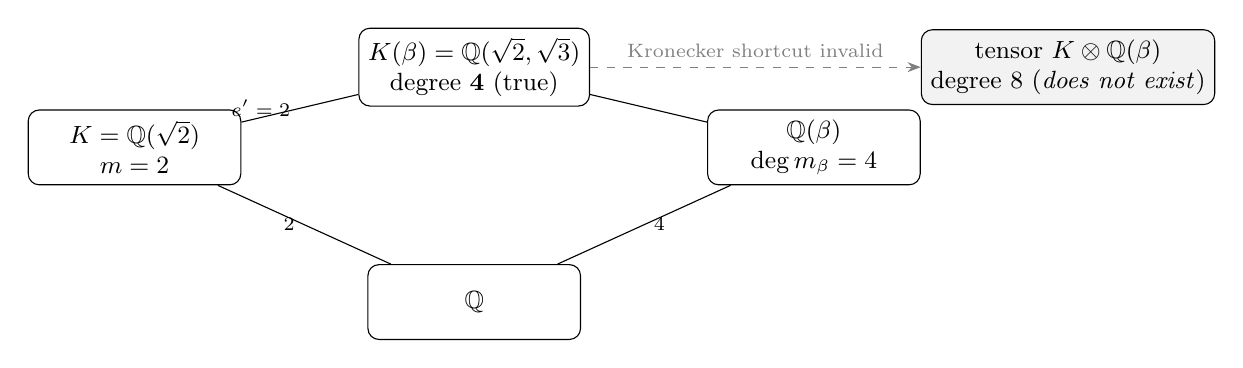
\begin{tikzpicture}[
  fld/.style={draw, rounded corners, align=center, minimum width=2.7cm, minimum height=0.95cm, font=\small},
  >={Stealth[]}, node distance=8mm and 16mm]
  \node[fld] (Q) {$\Q$};
  \node[fld, above left=10mm and 16mm of Q] (K) {$\K=\Q(\sqrt2)$\\$m=2$};
  \node[fld, above right=10mm and 16mm of Q] (B) {$\Q(\beta)$\\$\deg m_\beta=4$};
  \node[fld, above=20mm of Q] (T) {$\K(\beta)=\Q(\sqrt2,\sqrt3)$\\degree $\mathbf 4$ (true)};
  \node[fld, right=42mm of T, fill=black!5] (X) {tensor $\K\otimes\Q(\beta)$\\degree $8$ (\emph{does not exist})};
  \draw[-] (Q) -- (K) node[midway,left,font=\scriptsize]{$2$};
  \draw[-] (Q) -- (B) node[midway,right,font=\scriptsize]{$4$};
  \draw[-] (K) -- (T) node[midway,left,font=\scriptsize]{$e'=2$};
  \draw[-] (B) -- (T);
  \draw[->, dashed, gray] (T) -- (X) node[midway,above,font=\scriptsize]{Kronecker shortcut invalid};
\end{tikzpicture}
\caption{The non-disjoint witness of Example~\ref{ex:nondisjoint}. Because $m_\beta=x^4-10x^2+1$ factors over
$\K=\Q(\sqrt2)$ (so $e'=[\K(\beta):\K]=2$), the true compositum $\Q(\sqrt2,\sqrt3)$ has degree $m e'=4$, not
the tensor degree $m\deg m_\beta=8$; the disjoint Kronecker Gram $\GG_\K\otimes\GG_{\Q(\beta)}$ would describe
an $8$-dimensional space that does not exist. The construction selects $m_\theta=x^4-22x^2+25$ from the
degree-$6$ operator polynomial, machine-verified.}
\label{fig:nondisjoint}
\end{figure}

\begin{remark}[Honest scope of the non-disjoint construction]\label{rem:nondisjoint-scope}
This resolves the construction in the \emph{bounded-degree} regime: the factorisation over $\Q$ is a Kronecker
method capped at degree $12$, above which the learner refuses (rather than producing a fictitious Gram) and
flags a Zassenhaus/$p$-adic upgrade as future work. So the open problem O4 of~\cite{VectorSubstrate} is
\emph{advanced and machine-verified in the bounded case}, not settled in full generality. We classify the
witness as \emph{exact-computed} (Table~\ref{tab:ledger}).
\end{remark}

\section{Capacity and the applied growth gate}\label{sec:capacity}

The substrate paper proves the static admissibility theory; here we report the gate as \emph{implemented} and
its principled, opt-in tightening.

\subsection{The exact Northcott gate}
A monic-integer minimal polynomial $m$ is \emph{admissible} for a budget $(D_{\max},H_{\max})$ iff
$\deg m\le D_{\max}$ and $\ch(m)=\max_i|c_i|\le H_{\max}$; the admissible set is finite (Northcott), and the
decision is made on \emph{integers only}~\cite[Prop.~5.5]{VectorSubstrate}. The shipped
\texttt{capacity\_decision} returns one of $\textsc{grow}/\textsc{stop}/\textsc{reject}$: \textsc{stop} if the
residual norm is at or below a floor (defect captured / noise); else \textsc{reject} if inadmissible; else
\textsc{grow}. The float Mahler measure never crosses the boundary---a float coefficient, even an
integer-valued one, is refused at the gate.

\begin{example}[The gate decides on exact integers]\label{ex:gate}
The seed $2\sqrt6$ ($x^2-24$) has $(\deg,\ch)=(2,24)$ and $\sum c_i^2=577$, certifying $\Mah^2\le577$ by
Landau with no root. Under $\mathrm{Budget}(64,256)$ and gain $96$ the decision is \textsc{grow}; under
$\mathrm{Budget}(4,10)$ it is \textsc{reject} ($24>10$); with gain $0$ it is \textsc{stop}. The seed $\sqrt7$
($x^2-7$, $\sum c_i^2=50$) certifies $\Mah\le8$ exactly ($50\le64$) while the float Mahler is
$7.0000000000\ldots$; the integer gate is invariant to that rounding noise. Machine-verified
(\texttt{test\_capacity.py}, commit \texttt{c8fdb8a}).
\end{example}

\subsection{The Fisher reading and the degree-aware floor}
The substrate proves that on the trace-zero (residual) subspace the trace form is degree-scaled Fisher
information, $\lVert\rr\rVert_\GG^2=n\,\Fish_{\mathrm{exp}}(\rr)$, provided $1\in\col(\BB)$
(so $\Tr(\rr)=0$)~\cite[Lem.~7.9, Thm.~7.11]{VectorSubstrate}. The implementation re-verifies the underlying
matrices exactly and uses the identity to make a growth floor \emph{degree-aware}.

\begin{example}[Exact Fisher matrices]\label{ex:fisher}
With $G=M\transpose M$ and $\Fish_{\mathrm{exp}}=\tfrac1n\big(\GG-\tfrac1n t t\transpose\big)$
($t$ the trace vector):
\[
\begin{array}{lll}
  \Q(\sqrt5),\ \{1,\varphi\}: & \GG=\big(\begin{smallmatrix}2&1\\1&3\end{smallmatrix}\big), &
    \Fish_{\mathrm{exp}}=\big(\begin{smallmatrix}0&0\\0&5/4\end{smallmatrix}\big);\\[3pt]
  \Q(\sqrt2,\sqrt3): & \GG=\diag(4,8,12,24), & \Fish_{\mathrm{exp}}=\diag(0,2,3,6);\\[2pt]
  \Q(\sqrt2,\sqrt3,\sqrt7): & \GG=\diag(8,56,16,112,24,168,48,336), & \Fish_{\mathrm{exp}}=\diag(0,7,2,14,3,21,6,42).
\end{array}
\]
For the residual $\sqrt5=2\varphi-1=(-1,2)$ (trace-zero), $\lVert\sqrt5\rVert_\GG^2=10=2\cdot5=n\,\Fish(\sqrt5)$
with $n=2$. On every trace-zero direction $\GG=n\,\Fish_{\mathrm{exp}}$---a \emph{subspace} identity, not a
full-matrix one: $\Fish_{\mathrm{exp}}$ and $\tfrac1n\GG$ agree on the trace-zero directions but differ at the
constant ($\Fish_{\mathrm{exp}}$ vanishes there, while $\tfrac1n\GG$ does not), which is exactly why the
identity requires $1\in\col(\BB)$. Machine-verified, both directions
(\texttt{test\_a3p2\_fisher.py}, commit \texttt{d526098}).
\end{example}

\begin{remark}[The applied threshold, with an honest reciprocity caveat]\label{rem:threshold}
The opt-in information threshold (default \emph{off}; with it off the gate returns the shipped verdict
byte-for-byte and imports no interval-arithmetic library) tests gain $\lVert\rr\rVert_\GG^2$ against cost
$\lambda\log\Mah(\theta)$ and a floor. The floor branch keys on whether the seed is \emph{reciprocal}:
\begin{itemize}[leftmargin=*]
  \item \emph{Non-reciprocal} seed: the floor is Smyth's $\mu_S=1.32471795724\ldots$ (real root of $x^3-x-1$),
        a \emph{theorem}~\cite{Smyth}; stored as a certified rational bracket. With $\lambda=2$ the constant
        floor is $2\log\mu_S=0.5623991486\ldots$, the degree-aware floor $n\cdot2\log\mu_S$ is $2.2496$ at
        $n=4$ and $4.4992$ at $n=8$.
  \item \emph{Reciprocal} seed (Salem numbers, units---which arise naturally): there is \emph{no proven uniform
        positive floor} (the unsolved core of Lehmer's problem); the gate falls back to Dobrowolski's
        degree-dependent bound~\cite{Dobrowolski}, which is vacuous at small degree. This caveat is explicit
        in the code and the tests, and is recorded as \emph{open} in Table~\ref{tab:ledger}.
\end{itemize}
The threshold \emph{subsumes} the shipped growth cases (gain $96,56\gg$ cost), and the degree-aware floor is
what differs from the floor-$0$ shipped gate on lattice-aligned sub-threshold noise. Machine-verified
(\texttt{test\_capacity\_threshold.py}, \texttt{test\_a3p2b\_threshold.py}, commits \texttt{c8fdb8a},
\texttt{c5605d7}); the exchange rate is no longer a posited scalar but the derived identity $\lambda=2c$
(Theorem~\ref{thm:lambda2c}), with $c$ the conformal constant of the declared generative model. The shipped
$\lambda=2$ is its Model--1 ($c=1$, Gaussian) instance; the degree--aware floor $n\cdot2\log\mu_S$ above is its
Model--2 ($c=n$) instance, so the two floor families of this remark are the two conformal readings of one
identity (Remark~\ref{rem:floorsunify}).
\end{remark}

\begin{example}[A certified \textsc{grow}, no trust in a rounded value]\label{ex:certified}
The information half of the threshold is intrinsically analytic ($\log\Mah$ is transcendental), but a
\emph{decision} can still be certified: an exact rational gain need only dominate a rigorous \emph{upper} bound
on the cost. For $\sqrt7$ ($x^2-7$, $\Mah=7$) at $\lambda=2$, interval arithmetic gives
$\log 7\in[1.94591,\,1.94592]$, so $\lambda\log 7\le 2\cdot1.94592=3.89184$, and the exact gain
$\lVert\rr\rVert_\GG^2=56$ satisfies $56\ge 3.89184\ge\lambda\log7$: \textsc{grow} is certified with no trust in
any rounded value. The same procedure certifies $2\sqrt6$ ($x^2-24$): $\log 24\in[3.17805,\,3.17806]$ gives
$\lambda\log24\le6.35612\le96$. By contrast, lattice-aligned noise of exact magnitude $\tfrac1{10}$ is
\textsc{stop}ped by the Smyth constant floor, $\tfrac1{10}<0.5624$. The enclosures are produced by
\emph{verified interval arithmetic} (\texttt{mpmath.iv}, the same discipline as the implementation's gate),
not by a trusted rounded $\log$: the companion probe asserts the exact rational gain dominates the rigorous
interval \emph{upper} bound (\texttt{test\_certified\_grow\_enclosures}, \S\ref{sec:appendix}), and the
production threshold is exercised by \texttt{test\_capacity\_threshold.py} (commit \texttt{c8fdb8a}).
\end{example}

\begin{remark}[Exactness has a price, but never changes a decision]\label{rem:cost}
Every gate quantity above is exact integer or rational arithmetic, trading floating speed for
reproducibility. The standing practical caveat is rational coefficient growth: exact Gram and projector entries
can acquire large numerators and denominators, so an implementation bounds the working degree and height
(which the capacity gate already enforces) or tests equalities modulo a prime and lifts. The only inexact step
anywhere is the threshold comparison against $\log\Mah$, handled by the certified enclosure of
Example~\ref{ex:certified} while the gain side stays an exact rational. None of this alters a decision---it
only prices exactness.
\end{remark}

\subsection{The exchange rate, derived: \texorpdfstring{$\lambda=2c$}{lambda = 2c}}\label{subsec:lambda}

The threshold of Remark~\ref{rem:threshold} compares a \emph{gain} $\lVert\rr\rVert_\GG^2$ against a \emph{cost}
$\lambda\log\Mah(\theta)$. We now show the rate $\lambda$ is not a free knob: reading the trace form as a Fisher
metric turns ``grow iff gain $\ge$ cost'' into a two--part minimum--description--length (MDL) code
\cite{Rissanen}, and the rate falls out as an identity. This closes open problem (O1) of \S\ref{sec:open} and,
together with \v{C}encov's theorem, recasts (O4) precisely.

\begin{theorem}[The exchange rate is twice the conformal constant]\label{thm:lambda2c}
Read the trace form as the Fisher metric $\Fish=\GG/c$ of the declared generative model---$c=1$ for the
Gaussian location family $\mathcal N(Ma,I_n)$ and $c=n$ for the maximum--entropy family on the Galois conjugates
restricted to the trace--zero subspace, the two readings established in~\cite{VectorSubstrate}. For a residual
$\rr$, the second--order expansion of the Kullback--Leibler divergence between the captured model and the model
that also explains $\rr$ is
\begin{equation}\label{eq:kl2c}
  D_{\mathrm{KL}}=\tfrac12\,\rr\transpose\Fish\,\rr=\frac1{2c}\,\lVert\rr\rVert_\GG^2 .
\end{equation}
The two--part MDL balance ``adjoin a direction iff the bits it explains meet the bits it costs,''
$D_{\mathrm{KL}}\ge\log\Mah(\theta)$, is therefore \emph{exactly} the threshold
$\lVert\rr\rVert_\GG^2\ge\lambda\log\Mah(\theta)$ of Remark~\ref{rem:threshold}, with
\begin{equation}\label{eq:lambda2c}
  \boxed{\;\lambda=2c\;}.
\end{equation}
The ``$2$'' is the structural $\tfrac12$ of the quadratic KL expansion, inverted; it is not a parameter. The
entire residual freedom is the conformal constant $c$.
\end{theorem}
\begin{proof}
The Fisher information is the Hessian of $D_{\mathrm{KL}}$ at the matching point, so the second--order term of
the expansion in a parameter perturbation $\delta$ is $\tfrac12\delta\transpose\Fish\,\delta$: the zeroth--order
term vanishes, and the first--order term vanishes because the score has mean zero, so the leading nonzero term
is quadratic. Setting $\delta=\rr$ and $\Fish=\GG/c$ gives~\eqref{eq:kl2c} (for the Gaussian location family the
expansion is \emph{exact}, KL being already quadratic). Substituting into $D_{\mathrm{KL}}\ge\log\Mah$ and
clearing the factor $\tfrac1{2c}$ yields $\lVert\rr\rVert_\GG^2\ge 2c\log\Mah$, i.e.\ $\lambda=2c$. The per--seed
entropy $\log\Mah$ is the description length of the adjoined direction (the topological entropy of the companion
toral automorphism, Lind--Schmidt--Ward~\cite{LSW}); it is the \emph{cost} ledger and does not enter $\lambda$,
which is purely the unit conversion between the gain $\lVert\rr\rVert_\GG^2$ and the explained divergence
$D_{\mathrm{KL}}$.
\end{proof}

\begin{remark}[The two shipped floors are the two readings of $\lambda=2c$]\label{rem:floorsunify}
Remark~\ref{rem:threshold} already carries both instances. The \emph{constant} floor $2\log\mu_S=0.5623991\ldots$
is the Model--1 value $\lambda=2$ ($c=1$); the \emph{degree--aware} floors $n\cdot2\log\mu_S$ ($2.2496$ at $n=4$,
$4.4992$ at $n=8$) are the Model--2 value $\lambda=2n$ ($c=n$). The single expression $2c\log\mu_S$ evaluated at
$c\in\{1,n\}$ reproduces both, so the paper's two floor families were never independent choices: they are the two
conformal readings of one identity. (Verified: the floors recompute to $0.5624,2.2496,4.4992$ from $\mu_S$, the
root of $x^3-x-1$, in the companion derivation check of \S\ref{sec:appendix}.)
\end{remark}

\begin{remark}[The residual freedom is the conformal scale, and it is irreducible]\label{rem:cencov}
Theorem~\ref{thm:lambda2c} replaces the posited scalar $\lambda$ by the identity $\lambda=2c$, leaving a
\emph{single} free quantity: the conformal constant $c$. By \v{C}encov's theorem the Fisher metric is the unique
Riemannian metric invariant under sufficient statistics only \emph{up to a positive scale} \cite{Cencov}; that
scale is precisely $c=\lambda/2$. Hence no invariance principle internal to information geometry can fix $c$:
this is an impossibility result, not a missing lemma, and it is exactly the content of the no--canonical--model
conjecture of~\cite{VectorSubstrate}. Two readings of the field's own structure already name two values: $c=1$, under which
the Jeffreys information volume equals $\sqrt{\det\GG}=\sqrt{|d_\K|}$ (the field discriminant)~\cite{Jeffreys,
VectorSubstrate}, and $c=n$, under which per--conjugate significance is degree--invariant. Choosing $c$ is
choosing a generative model; it is a declared modeling commitment. Definition~\ref{def:frameshift} adds a third
value, native not to an external prior but to the geometry of a critical point.
\end{remark}

We make the critical--point reading precise through the self--action of the $C$--ladder, the quadratic family
$x^2+x=C$ whose discriminant $1+4C$ controls the keystone (the golden case $C=1$ gives discriminant $5$).

\begin{proposition}[Self--action spectrum of the $C$--ladder]\label{prop:trifurcation}
For $C\in\Q$ let $R_C=\big(\begin{smallmatrix}0&C\\1&-1\end{smallmatrix}\big)$ be the companion matrix of
$x^2+x-C$, with eigenvalues $(-1\pm\sqrt{1+4C})/2$. The Lie self--action $X\mapsto[R_C,X]=R_CX-XR_C$ on
$M_2(\Q)$ has spectrum
\begin{equation}\label{eq:trifurcation}
  \big\{\,-\sqrt{1+4C},\;\,0,\;\,+\sqrt{1+4C}\,\big\}\qquad(\text{the }0\text{ with multiplicity }2),
\end{equation}
its nonzero eigenvalues being the difference of the two eigenvalues of $R_C$. The $0$--eigenspace is the
centraliser $\spn\{I,R_C\}$. At the golden value $C=1$ the spectrum is $\{-\sqrt5,0,+\sqrt5\}$ with
$\sqrt5=\varphi-\psi$, and $R_1$ is conjugate to the keystone $R=\big(\begin{smallmatrix}0&1\\1&1\end{smallmatrix}\big)$
($\charpoly=x^2-x-1$; both have discriminant $5$, hence the same self--action gap).
\end{proposition}
\begin{proof}
For a $2\times2$ matrix with eigenvalues $\{a,b\}$ the adjoint action has eigenvalues $\{a-a,a-b,b-a,b-b\}=
\{0,0,\pm(a-b)\}$; here $a-b=\sqrt{1+4C}$. The centraliser of a non--scalar $2\times2$ matrix is the
two--dimensional algebra $\spn\{I,R_C\}$, which is the kernel of the action. The golden specialisation is
$1+4\cdot1=5$, and $\varphi-\psi=\tfrac{1+\sqrt5}2-\tfrac{1-\sqrt5}2=\sqrt5$.
\end{proof}

The three eigen--channels of~\eqref{eq:trifurcation} are exactly the growth decision read in the eigenframe:
$+\sqrt{1+4C}$ is the off--diagonal \emph{growth} channel (\textsc{grow}), $-\sqrt{1+4C}$ the decay channel
(\textsc{stop}), and the marginal $0$--channel $\spn\{I,R_C\}$ is the captured, residual--zero direction. This is
the structure that fixes the conformal scale at a critical point.

\begin{definition}[The critical--point (frame--shift) canonicalization]\label{def:frameshift}
At a critical value $C$ of the ladder, read the growth decision in the eigenframe of the self--action
$[R_C,\cdot]$. Its intrinsic scale is the spectral gap $\sqrt{1+4C}$ of Proposition~\ref{prop:trifurcation}---the
distance from the captured ($0$) channel to the growth/decay channels, and also $\sqrt{\Mah(\sqrt{1+4C})}$ since
$\Mah(x^2-(1+4C))=1+4C$. Equating the decision scale $\lambda C$ with this gap,
\begin{equation}\label{eq:frameshift}
  \lambda\,C=\sqrt{1+4C}\quad\Longrightarrow\quad
  \lambda=\frac{\sqrt{1+4C}}{C},\qquad c=\frac{\lambda}{2}=\frac{\sqrt{1+4C}}{2C},
\end{equation}
fixes the conformal constant at the gate. At the golden gate $C=1$ this is $c=\sqrt5/2$, $\lambda=\sqrt5$---the
exchange rate \emph{is} the spectral gap.
\end{definition}

\begin{table}[t]\centering
\small
\begin{tabular}{llll}
\toprule
Canonicalization & principle & $c$ & status \\
\midrule
Model 1 & Jeffreys volume $\sqrt{\det\GG}=\sqrt{|d_\K|}$ & $1$ & declared \cite{Jeffreys} \\
Model 2 & degree--invariant per--conjugate significance & $n$ & declared \\
Critical point & self--action eigenframe scale (gap $\sqrt{1+4C}$) & $\sqrt{1+4C}/(2C)$ & declared; framework--native \\
\bottomrule
\end{tabular}
\caption{The conformal constant $c$ under three canonicalizations, all giving $\lambda=2c$ by
Theorem~\ref{thm:lambda2c}. By \v{C}encov's theorem (Remark~\ref{rem:cencov}) none is forced by invariance; the
third is selected by the geometry of a critical point (Definition~\ref{def:frameshift}), and at the golden gate
gives $c=\sqrt5/2$, $\lambda=\sqrt5$. On the ladder gates $C\in\{\tfrac14,\tfrac12,1\}$ the gap is
$\sqrt{1+4C}\in\{\sqrt2,\sqrt3,\sqrt5\}$, the three irrationals $\sqrt{\Mah(\sqrt2)},\sqrt{\Mah(\sqrt3)},
\sqrt{\Mah(\sqrt5)}$.}
\label{tab:canon}
\end{table}

\begin{remark}[What is closed, and what is a declared choice]\label{rem:lambdaclose}
The identity $\lambda=2c$ is \emph{forced} (Theorem~\ref{thm:lambda2c}): the exchange rate is no longer free, and
(O1) and (O4) of \S\ref{sec:open} are one degree of freedom, related by $\lambda=2c$. What remains is not a
\emph{value} but a \emph{model}: which $c$ in Table~\ref{tab:canon} the application declares. \v{C}encov's theorem
guarantees this cannot be reduced further by invariance. The critical--point value $\sqrt{1+4C}/(2C)$ is the one
the substrate's own structure supplies---the eigenframe's intrinsic scale rather than an imported prior---but it
is, per \v{C}encov, a principled \emph{choice}, not a derivation. Operationally the choice is immaterial on the
shipped seeds: their gains $96,56$ exceed every floor for all $c\in[1,n]$, so the shipped \textsc{grow}/\textsc{stop}
verdicts are invariant across the named models (it would matter only for a seed whose gain lands in the band
$(2\log\mu_S,\,2n\log\mu_S)$).
\end{remark}

\begin{remark}[The discriminant flip and the totally--real hypothesis]\label{rem:flip}
The gap $\sqrt{1+4C}$ is real precisely when $1+4C>0$. The discriminant $D=1+4C$ crosses zero at $C=-\tfrac14$
(a double root), and for $D<0$ the eigenvalues of $R_C$ become complex conjugates on a circle: the $\pm$ channels
of~\eqref{eq:trifurcation} turn from real growth/decay into imaginary rotation $\pm i\sqrt{|D|}$, while the
captured $0$--channel persists. This is the same sign that governs the metric: the trace form of $\Q(\sqrt D)$ is
positive definite (a Fisher metric) for $D>0$ (totally real) and indefinite for $D<0$ (a complex place), which is
why the Fisher reading of \S\ref{subsec:lambda} and~\cite{VectorSubstrate} requires the totally--real hypothesis.
The conformal canonicalization of Definition~\ref{def:frameshift} therefore lives on the $D>0$ side; the
$D<0$ regime is a rotation, not a growth, and is recorded as out of scope here.
\end{remark}

\section{The automatic learning loop}\label{sec:loop}

The pieces above are driven automatically by a calibration-gated detector that never auto-acts, and a
field-growing learner that measures its own gain.

\subsection{A calibration-gated detector}
The detector scores each exact observation by the residual norm $s=\lVert\rr\rVert_\GG^2$ and raises an
\emph{anomaly} only when $s>$ threshold \emph{and} a calibration predicate passes; it then surfaces a growth
\emph{proposal} (a \texttt{SeedProposal} in-field, a \texttt{FieldExtensionProposal} out-of-field), never
auto-confirming. Formally $\texttt{anomaly}=\texttt{novel}\wedge\texttt{calibrated}$, and the wrapped models'
basis size and field degree are invariant until an explicit caller confirm.

\begin{proposition}[Propose, never auto-grow]\label{prop:detector}
For an in-distribution stream (every observation in $\col(\BB)$) the score is $0$ and nothing is surfaced.
For a persistent off-axis novelty the score is positive; while uncalibrated the novelty is recorded but the
alert is \emph{suppressed} and no proposal surfaces; once calibrated the same observation alerts and surfaces
a proposal. Scoring and surfacing leave the wrapped models unchanged. Surfaced proposals are appended to a
$\mathrm{SHA}\text{-}256$ witness chain~\eqref{eq:chain}.
\end{proposition}
\begin{proof}
Each clause is a machine-checked assertion:
\texttt{test\_a7\_in\_distribution\_stream\_no\_anomaly} (score $0$, nothing surfaced),
\texttt{test\_a7\_calibration\_gate\_suppresses\_until\_calibrated},
\texttt{test\_a7\_proposes\_but\_never\_auto\_grows}, and
\texttt{test\_a7\_witness\_of\_surfaced\_proposals} (verify \texttt{True}; tamper a recorded score and verify
flips \texttt{False}); commits \texttt{6ad20eb}, \texttt{038ee27}.
\end{proof}

\begin{remark}[What ``calibration'' is, precisely---and what it is not]\label{rem:calibration}
The calibration predicate is an \emph{injected} gate, and the shipped constructor default is \emph{permissive}
(it admits once persistence is met). So ``calibration-gated'' names the \emph{mechanism}---detection is
decoupled from alerting through an explicit gate---not a substantive default policy; we say so plainly rather
than imply a calibration the default does not perform. A concrete, exact instance is provided and tested,
\texttt{variance\_calibration}, which opens only once the off-axis accumulator has both warmed up \emph{and}
\emph{settled}: its accumulated per-coordinate Welford variance $\sum_i M2_i$ (previously computed but unused)
lies within a declared fraction $\tau$ of the centroid's squared magnitude,
\begin{equation}\label{eq:calib}
  \textstyle\sum_i M2_i \;\le\; \tau\,n\sum_i \mathrm{mean}_i^2 ,
\end{equation}
all exact Fraction. This is distinct from persistence: persistence tests that the residual \emph{direction}
holds (the alignment test of Algorithm~\ref{alg:learn}), calibration that its \emph{magnitude} has settled, so
an aligned-but-volatile stream persists yet stays uncalibrated and surfaces no proposal. Machine-verified by
\texttt{test\_calibration.py} (a stable stream calibrates after warm-up; a volatile $1{\times}/10{\times}$
stream persists but is blocked from proposing; commit \texttt{1366d1c}).
\end{remark}

\begin{example}[A streaming detector trace]\label{ex:stream}
In the ambient $\K=\Q(\sqrt2+\sqrt3)$ with forced basis $\BB=\{1,\theta\}$ and a calibration predicate that
opens after the third observation, the off-axis $2\sqrt6=\theta^2-5$ carries the exact score $96$, and an
in-span observation scores $0$:
\begin{center}
\begin{tabular}{clccl}
\toprule
$t$ & observation & $\lVert\rr\rVert_\GG^2$ & calibrated & action \\
\midrule
$1$ & $2-\theta$ \ (in $\col\BB$)   & $0$  & no  & --- \\
$2$ & $3+4\theta$ \ (in $\col\BB$)  & $0$  & no  & --- \\
$3$ & $1+2\sqrt6$ \ (off-axis)      & $96$ & no  & novelty recorded, alert \emph{suppressed} \\
$4$ & $1+2\sqrt6$                   & $96$ & yes & alert; \emph{propose} seed $x^2-24$ \\
$5$ & confirm                       & ---  & yes & basis grows to $\{1,\theta,2\sqrt6\}$; witnessed \\
$6$ & $1+2\sqrt6$                   & $0$  & yes & captured \\
\bottomrule
\end{tabular}
\end{center}
The score is an exact rational at every step; the basis is mutated only at $t=5$, and only by an explicit
\emph{confirm}; steps $3$--$4$ show calibration decoupling detection from alerting, and step $6$ shows capture
collapsing the score to $0$. Machine-verified by the detector tests (commit \texttt{6ad20eb}).
\end{example}

\subsection{Detector-driven gain and the full loop}
The seam that makes the loop automatic is that the growth \emph{gain} is not supplied by the caller but
\emph{measured}: the field-growing learner computes the exact out-of-field residual and that value \emph{is}
the gain.

\begin{theorem}[The automatic loop returns the residual to zero]\label{thm:loop}
Starting from $\K=\Q(\sqrt2)$ with $\BB=\{1\}$ (so $1\in\col(\BB)$, degree $2$), the loop
\[
  \text{detect}\ \to\ \text{auto-gain}\ \to\ \text{propose}\ \to\ \text{gate}(\text{effective degree})\ \to\
  \text{confirm}\ \to\ \text{re-home onto }\Q(\theta)\ \to\ \rr=\mathbf 0
\]
captures an out-of-field $\beta=\sqrt2+\sqrt3$: the auto-gain equals the measured residual, the gate judges
the \emph{true} compositum degree $4$ (Definition~\ref{def:effdeg}), and after confirm the basis is re-homed
into the power basis of the primitive $\theta$ with $m_\theta=x^4-22x^2+25$, returning the residual to $0$
exactly. \emph{confirm} is the sole field-growth mutator; \emph{propose} leaves the degree unchanged.
\end{theorem}
\begin{proof}
The auto-gain is the exact field-residual: an exact \texttt{Fraction} (value $12$ for the witness), and
scaling the observed element by $2$ scales it quadratically to $48$, confirming it is a genuine norm rather
than a tag. The gate uses $\texttt{effective\_degree}=m e'=4$, so $\mathrm{Budget}(D_{\max}=4)$ grows while
$\mathrm{Budget}(D_{\max}=3)$ refuses with \texttt{capacity\_reject}. Re-homing recomputes each forced column
in the power basis of $\theta$ (Theorem~\ref{thm:nondisjoint}) and clears denominators
(Lemma~\ref{lem:rehome}); the captured directions then have residual $0$. Machine-verified end-to-end by
\texttt{test\_e2e\_out\_of\_field\_residual\_driven\_to\_zero\_through\_learner},
\texttt{test\_seam\_detector\_residual\_is\_the\_growth\_gain},
\texttt{test\_auto\_gain\_equals\_measured\_residual}, and
\texttt{test\_effective\_degree\_is\_true\_compositum\_degree} (commits \texttt{038ee27}, \texttt{ef3b86d}).
\end{proof}

\begin{figure}[ht]
\centering
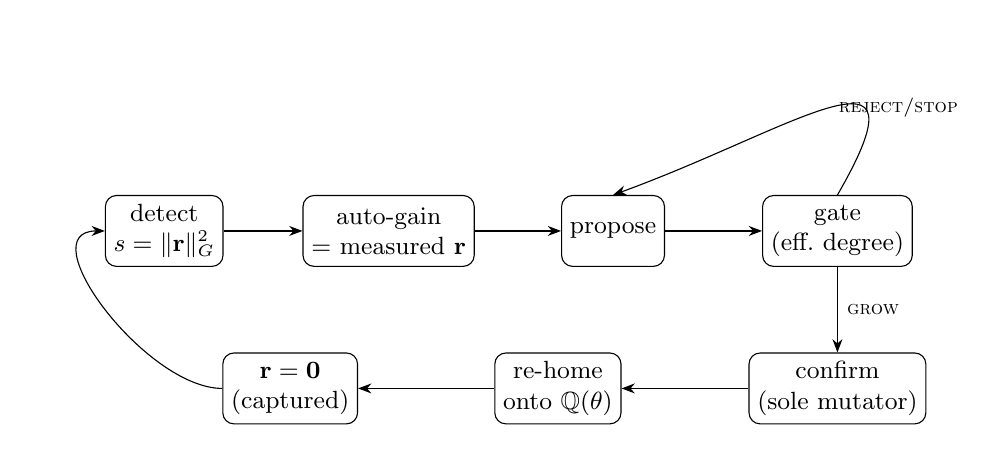
\begin{tikzpicture}[
  lp/.style={draw, rounded corners, align=center, font=\small, minimum height=0.9cm, inner sep=3pt},
  >={Stealth[]}]
  \node[lp] (d) at (0,0) {detect\\$s=\lVert\rr\rVert_\GG^2$};
  \node[lp] (g) at (2.85,0) {auto-gain\\$=$ measured $\rr$};
  \node[lp] (p) at (5.7,0) {propose};
  \node[lp] (gate) at (8.55,0) {gate\\(eff.\ degree)};
  \node[lp] (c) at (8.55,-2.0) {confirm\\(sole mutator)};
  \node[lp] (rh) at (5.0,-2.0) {re-home\\onto $\Q(\theta)$};
  \node[lp] (z) at (1.6,-2.0) {$\rr=\mathbf 0$\\(captured)};
  \draw[->] (d)--(g); \draw[->] (g)--(p); \draw[->] (p)--(gate);
  \draw[->] (gate)--(c) node[midway,right,font=\scriptsize]{\textsc{grow}};
  \draw[->] (c)--(rh); \draw[->] (rh)--(z);
  \draw[->] (z) to[out=180,in=180] (d.west);
  \draw[->] (gate.north) to[out=60,in=20,looseness=2.2] node[right,font=\scriptsize]{\textsc{reject}/\textsc{stop}} (p.north);
\end{tikzpicture}
\caption{The automatic loop of Theorem~\ref{thm:loop}. The detector's measured residual \emph{is} the growth
gain; the gate judges the \emph{true} compositum degree (Definition~\ref{def:effdeg}); \emph{confirm} is the
sole mutator; re-homing onto the primitive element's power basis returns the residual to $0$. The gate may
instead \textsc{reject} (inadmissible) or \textsc{stop} (sub-floor), leaving the model unchanged.}
\label{fig:loop}
\end{figure}

\begin{algorithm}[ht]
\DontPrintSemicolon
\KwIn{ambient $\K=\Q(\alpha)$, forced basis $\BB$ with $1\in\col(\BB)$, an out-of-field stream; budget}
\For{each observation $\xx$}{
  $s \gets \lVert \xx - P\xx\rVert_\GG^2$ \tcp*{detect: exact residual score}
  \If{$s>0$ \textnormal{\textbf{and} calibrated}$()$}{
    $g \gets \textnormal{measuredFieldResidual}(\xx)$ \tcp*{auto-gain $=$ the MEASURED out-of-field residual}
    $(\beta,m_\beta) \gets \textnormal{candidateGenerator}(\xx)$\;
    factor $m_\beta$ over $\K$; \ $e' \gets$ degree of the $\K$-factor satisfied by $\beta$ \tcp*{effective degree}
    \uIf{$\textnormal{capacity}\big(\,\cdot\,,\,g,\ \textnormal{budget on } [\K:\Q]\,e'\,\big)=\textsc{grow}$}{
      $\theta' \gets$ primitive element of $\K(\beta)$; \ $m_{\theta'}\gets$ its minpoly \tcp*{Thm.~\ref{thm:nondisjoint}}
      re-home each column of $\BB$ into the power basis of $\theta'$ (clear denominators, Lem.~\ref{lem:rehome})\;
      \textnormal{confirm} \tcp*{$\blacktriangleleft$ sole field-growth mutation; afterwards $\lVert\xx-P\xx\rVert_\GG^2=0$}
    }
    \lElse{\textsc{reject}/\textsc{stop}: surface a proposal, do not grow}
  }
}
\caption{The automatic detector-driven loop (\S\ref{sec:loop}, Theorem~\ref{thm:loop}). The gain is
\emph{measured}, not supplied; the gate judges the \emph{true} compositum degree $[\K:\Q]\,e'$ (not the tensor
degree); \emph{confirm} is the sole field-growth mutation; re-home returns the residual to $0$ in $\Q(\theta')$.}
\label{alg:loop}
\end{algorithm}

\begin{lemma}[Re-home is projector-invariant under column scaling]\label{lem:rehome}
Re-homing a forced-basis column from $\K$ into $\Q(\theta)$ can produce fractional power-basis coordinates;
scaling a column to the smallest integer vector on the same line (clearing denominators) does not change
$\col(\BB)$, hence does not change the projector $P$ or any residual. In particular a captured direction stays
captured across the re-home.
\end{lemma}
\begin{proof}
$P=\BB(\BB\transpose\GG\BB)\inv\BB\transpose\GG$ depends only on $\col(\BB)$: replacing a column $b$ by $cb$
($c\in\Q^\times$) is the right-multiplication $\BB\mapsto\BB D$ by an invertible diagonal $D$, under which
$P$ is invariant ($P$ is the unique $\GG$-orthogonal projector onto $\col(\BB)$). Machine-checked by
\texttt{test\_rehome\_preserves\_subspace\_with\_a\_nontrivial\_basis} (commit \texttt{ef3b86d}).
\end{proof}

\begin{remark}[$1\in\col(\BB)$ survives growth]\label{rem:oneinB}
The constant $1=(1,0,\dots,0)$ is the zeroth power-basis vector in \emph{any} power basis, so $1\in\col(\BB)$
is preserved across the re-home into $\Q(\theta)$, keeping the Fisher precondition of
\S\ref{sec:capacity} valid in the grown field. Machine-checked by
\texttt{test\_one\_in\_basis\_preserved\_across\_growth} (commit \texttt{ef3b86d}). On this increment the
info-threshold is left off (floor $0$), so a tiny positive gain still grows; the principled floor is the
opt-in of Remark~\ref{rem:threshold}.
\end{remark}

\section{A residual-valued language}\label{sec:language}

We now exhibit the same residual-return mechanism as a \emph{language}, over the Clifford algebra
$\Cl(2,0)\cong M_2(\R)$, realised exactly over $\Q$ (\texttt{Fraction}, no float in any decision). This layer
lives in a separate, one-way module; it reads the number-field engine only through a $\varphi$-keystone
bridge and is never imported back.

\subsection{The exact carrier}
A \emph{holding} is $X=a\cdot 1+b\,e_1+c\,e_2+d\,i$ with $a,b,c,d\in\Q$, $e_1^2=e_2^2=1$, $i=e_1e_2$,
$i^2=-1$, and the matrix isomorphism $\mathrm{mat}(X)=\big(\begin{smallmatrix}a+c&b-d\\b+d&a-c\end{smallmatrix}\big)$.
The readings $\nu(X)=M(X)-X$ (idempotence defect, $M(X)=\tilde X X$ the Gram) and $R_K(X)=M(X)-\tau(M(X))\,1$
(trace-free Gram) are decided at zero tolerance: $\nu(P_0)=\VOID$ for the gate $P_0=\tfrac12(1+e_2)$,
$R_K(1)=\VOID$, $R_K(P_0)=\tfrac12 e_2\ne\VOID$, and $R_K^2=\VOID$ (bite-depth $\le2$). Cayley--Hamilton
$\Phi_X(X)=X^2-\tau(X)X+\det(X)\,1=\VOID$ holds exactly. Machine-verified
(\texttt{test\_holding.py}, commit \texttt{f925e50}; exact core \texttt{6cd3800}).

\begin{example}[The readings are zero-tolerance decisions]\label{ex:readings}
The gate $P_0=\tfrac12(1+e_2)$ is a symmetric idempotent: $\nu(P_0)=M(P_0)-P_0=\VOID$ exactly, so $P_0$ is
``captured'' by the idempotence reading, yet $R_K(P_0)=\tfrac12 e_2\ne\VOID$---it is not conformal, so the
trace-free Gram is a nonzero residual. By contrast $R_K(1)=\VOID$ (the unit is conformal). The type lattice is
exact: the keystone $R$ has $\tau(R)=\tfrac12,\ \det(R)=-1$, hence $\mathrm{TYPE}(R)=\{\text{gen}\}$ (it
satisfies the golden law $X^2=X+1$), while $P_0$ has $\mathrm{TYPE}(P_0)=\{\text{idem},\text{rest}\}$ and a
generic holding has empty type. Every one of these is an $==$ decision over $\Q$, machine-verified
(\texttt{test\_holding.py}, \texttt{test\_type\_lattice\_exact}, commits \texttt{f925e50}, \texttt{4817b62}).
\end{example}

\subsection{The $\varphi$-keystone return operator}
The keystone is $R=\tfrac12+e_1-\tfrac12 e_2$, i.e.\ $\mathrm{mat}(R)=\big(\begin{smallmatrix}0&1\\1&1\end{smallmatrix}\big)$,
the companion matrix of $x^2-x-1$. It satisfies the golden law $R^2=R+1$ (so $\mathrm{TYPE}(R)=\{\text{gen}\}$),
and $\mathrm{mat}(R)$ is symmetric. The \emph{return operator} is the Sylvester self-action
\begin{equation}\label{eq:Lop}
  \Lop(X)=RX+XR-X .
\end{equation}

\begin{proposition}[$\Lop$ is exact and oracle-checked]\label{prop:Lop}
$\Lop$ is computed by the exact geometric product and agrees on every sampled holding with an
\emph{independent} matrix-route oracle (own $\mathrm{mat}$/multiply/$\mathrm{cl}$, never calling the holding
product), ruling out a single-route bug. $R\notin\ker\Lop$ (indeed $\Lop(R)=\tfrac52+e_1-\tfrac12 e_2\ne\VOID$).
\end{proposition}
\begin{proof}
Machine-checked by \texttt{test\_L\_matches\_matrix\_oracle\_exact} and
\texttt{test\_keystone\_R\_not\_in\_kernel\_exact} (commit \texttt{4817b62}).
\end{proof}

\begin{theorem}[The exact kernel is the lexicon space]\label{thm:kernel}
$\ker\Lop$ is exactly two-dimensional, computed by hand-rolled rational Gaussian elimination on the $4\times4$
matrix of $\Lop$ over $\{1,e_1,e_2,i\}$ (not by floating SVD), with exact basis
\[
  \ker\Lop=\spn\{\,e_1+2e_2,\ \ i\,\}=\spn\{H(0,1,2,0),\,H(0,0,0,1)\}.
\]
The Sylvester eigenvalue argument confirms the dimension: $\Lop=S-\mathrm{id}$ where $S(X)=RX+XR$ has
eigenvalues $\lambda_a+\lambda_b$ over the eigenvalues $\{\varphi,\psi\}$ of $R$ (with $\varphi+\psi=1$), i.e.\
$\{2\varphi,1,1,2\psi\}$, so $\Lop$ has eigenvalue $0$ with multiplicity $2$.
\end{theorem}
\begin{proof}
The rational nullspace computation returns the stated integer-normalised basis; the eigenvalue count matches.
Machine-verified by \texttt{test\_kernel\_exact\_dim\_and\_basis} (commit \texttt{4817b62}).
\end{proof}

\begin{remark}[A corrected hint, pinned by its disproof]\label{rem:disproof}
An earlier design note claimed the antisymmetric generator ``$N=H(0,-1,1,0)$'' lay in $\ker\Lop$. This is
\emph{false}: $\Lop(H(0,-1,1,0))=H(-3,0,0,0)\ne\VOID$. The slip transcribed the four \emph{matrix} entries of
$N=\big(\begin{smallmatrix}0&-1\\1&0\end{smallmatrix}\big)$ directly into holding coordinates instead of
through the iso; the correct image is $\mathrm{cl}\big(\begin{smallmatrix}0&-1\\1&0\end{smallmatrix}\big)=i=H(0,0,0,1)$,
which \emph{is} in the kernel. The disproof is itself a machine-checked test
(\texttt{test\_corrected\_handoff\_hint\_is\_not\_in\_kernel}, commit \texttt{4817b62})---a small instance of
the discipline that load-bearing claims, including negative ones, are pinned by computation.
\end{remark}

\subsection{The commit, the word, and the growing lexicon}
The \emph{commit} is the exact idempotent orthogonal projector onto $\ker\Lop$, value-pinned (idempotence
alone is also satisfied by the identity, so the matrix is asserted, not merely $P^2=P$):
\begin{equation}\label{eq:proj}
  \mathrm{commit}=\text{proj}_{\ker\Lop}=
  \begin{pmatrix}0&0&0&0\\0&\tfrac15&\tfrac25&0\\0&\tfrac25&\tfrac45&0\\0&0&0&1\end{pmatrix}
  \quad(\text{in coordinates }1,e_1,e_2,i).
\end{equation}
A token's \emph{word} is a sign-aware sparse code over the kernel basis (an exact, $\mathrm{sqrt}$-free
$L^1$-relative threshold $\tau=\tfrac14$); sign discriminates antipodal rays, so $\mathrm{word}(i)=(\!+i)$ and
$\mathrm{word}(-i)=(\!-i)$ are opposite meanings.

\begin{theorem}[Generalisation by return-to-zero]\label{thm:generalise}
A learned dictionary value is exactly a committed residue: $\mathrm{commit}(X)\in\ker\Lop$, decided over $\Q$.
Tokens that commit to the \emph{same} exact residue share one lexicon entry; tokens with \emph{distinct}
residues stay distinct. Thus $E_1$ and $E_1+1$ merge (the constant $1$ is orthogonal to the slack, so
$\mathrm{commit}(E_1+1)=\mathrm{commit}(E_1)=H(0,\tfrac15,\tfrac25,0)$), and positive scaling preserves the
word ($\mathrm{word}(3E_1)=\mathrm{word}(E_1)$); but $i$ (value $H(0,0,0,1)$) and $2i$ (value $H(0,0,0,2)$),
though they share the word $(\!+i)$, are \emph{distinct} entries---dedup is on the exact value, not the coarse
sign-word. Lexicon identifiers are deterministic content hashes
$\mathrm{id}=\mathrm{SHA}\text{-}256(\text{canonical }\mathrm{Fraction}\text{ string})[0{:}16]$, order- and
run-independent.
\end{theorem}
\begin{proof}
Machine-verified by \texttt{test\_projector\_exact\_matrix\_value},
\texttt{test\_generalization\_same\_residue\_same\_value\_and\_word},
\texttt{test\_distinct\_residues\_stay\_distinct}, and
\texttt{test\_ids\_are\_deterministic\_and\_order\_independent} (commits \texttt{4817b62}, \texttt{d1312ed}).
\end{proof}

\begin{example}[A growing lexicon, traced]\label{ex:lexicon}
Feeding five tokens through \emph{acquire} (commit, then add) grows the lexicon to four entries: the constant
$1$ is orthogonal to the slack, so $E_1$ and $E_1+1$ return to the same value and merge; the pseudoscalar
$i$, its double $2i$, and its antipode $-i$ are three distinct exact values---even though $i$ and $2i$ share
the word $(\!+i)$.
\begin{center}
\begin{tabular}{llll}
\toprule
token $X$ & committed value $\in\ker\Lop$ & word & lexicon \\
\midrule
$E_1=(0,1,0,0)$    & $H(0,\tfrac15,\tfrac25,0)$ & $(\!+e_1{+}2e_2)$ & new entry $\#1$ \\
$E_1+1=(1,1,0,0)$  & $H(0,\tfrac15,\tfrac25,0)$ & $(\!+e_1{+}2e_2)$ & merged (same residue) \\
$i=(0,0,0,1)$      & $H(0,0,0,1)$               & $(\!+i)$          & new entry $\#2$ \\
$2i=(0,0,0,2)$     & $H(0,0,0,2)$               & $(\!+i)$          & new entry $\#3$ (same word, distinct value) \\
$-i=(0,0,0,-1)$    & $H(0,0,0,-1)$              & $(\!-i)$          & new entry $\#4$ (antipode) \\
\bottomrule
\end{tabular}
\end{center}
Five tokens, four entries: generalisation is collapse to a shared \emph{exact} residue, and the sign-word is a
label, not the dedup key. Machine-verified by the lexicon tests (commit \texttt{d1312ed}).
\end{example}

\subsection{The firewall, persistence, and the shell}
Statements carry a jurisdiction (Table~\ref{tab:firewall}), and only $\textsc{theorem}/\textsc{computed}$
cross a wire as fact; a learned lexicon entry is \textsc{computed}, never promoted to \textsc{theorem}.

\begin{table}[ht]
\centering
\small
\begin{tabular}{lccl}
\toprule
Jurisdiction & Wired? & Count in law bank & Meaning \\
\midrule
\textsc{theorem}          & yes & $20$ & proved (or exact-verified) fact \\
\textsc{computed}         & yes & $5$  & derived/learned (e.g.\ a lexicon entry, a reading) \\
\textsc{interpretive}     & no  & $2$  & glossed reading---returned only on explicit request, tagged \\
\textsc{false\_as\_stated} & no  & $0$  & defined for completeness; unused \\
\midrule
\textbf{wired total} & --- & $\mathbf{25}$ & what crosses by default ($20+5$) \\
\textbf{bank total}  & --- & $\mathbf{27}$ & all statements ($20+5+2$) \\
\bottomrule
\end{tabular}
\caption{The jurisdiction firewall of the language layer. \textsc{wired\_jurisdictions} $=
\{\textsc{theorem},\textsc{computed}\}$; the default surface returns the $25$ wired statements, the full
$27$ only on explicit request with each non-wired statement tagged. Machine-verified
(\texttt{test\_firewall}, \texttt{test\_math\_preserved}; commit \texttt{a5892c7}).}
\label{tab:firewall}
\end{table} The lexicon persists through a
$\mathrm{SHA}\text{-}256$ hash chain~\eqref{eq:chain} identical in form to the learner's, with exact
round-trip and tamper-evidence; and a JSON-in/JSON-out shell exposes the surface
(\texttt{read}/\texttt{render}/\texttt{observe}/\texttt{propose}/\texttt{commit}/\texttt{persist}/\texttt{restore})
under local-equivalence (in-process $=$ subprocess) and a robustness guard (a malformed request soft-errors,
never crashes). The whole layer is one-way disjoint: a scan finds the number-field repository references the
language module \emph{nowhere}, and only the keystone bridge reaches the live engine. The full suite is
\textbf{$121$ tests green} at the readiness tag \texttt{b1-ready} (commit \texttt{a5892c7}); the readiness gate
itself is mutation-proven load-bearing.

\section{The unifying principle and the \texorpdfstring{$\varphi$}{phi} keystone}\label{sec:unify}

\subsection{One mechanism, two instances}
The two faces are the same five-part structure (Table~\ref{tab:correspond}). The deepest shared piece is not
analogy but a literal identity: the witness chain~\eqref{eq:chain} is byte-identical in construction across the
learner and the lexicon, and capture is exact vanishing of a residual in both.

\begin{table}[ht]
\centering
\small
\begin{tabular}{lll}
\toprule
Role & Learning (number field $\K$) & Language ($\Cl(2,0)\cong M_2(\R)$) \\
\midrule
loss / residual & $\rr=\xx-P\xx$ (trace form $\GG$) & $\Lop(X)=RX+XR-X$ \\
captured $\iff$ & $\lVert\rr\rVert_\GG^2=0$ (exact, over $\Q$) & $\Lop(X)=\VOID$ (exact, over $\Q$) \\
landing space & $\col(\BB)\subseteq\K$ & $\ker\Lop=\spn\{e_1+2e_2,\,i\}$ \\
model state & forced basis $\BB$ (growing) & lexicon $\subseteq\ker\Lop$ (growing) \\
sole mutator & \emph{confirm} (adjoin seed) & \emph{commit} / lexicon \emph{add} \\
generalisation & same residual direction captured once & same exact residue $\Rightarrow$ one entry \\
witness & $\mathrm{SHA}\text{-}256$ chain~\eqref{eq:chain} & \emph{the same} $\mathrm{SHA}\text{-}256$ chain \\
exactness gate & $\Q/\Z$ decision; float refused & $\Q$ decision; float refused \\
\bottomrule
\end{tabular}
\caption{The residual-return correspondence. The two columns are one mechanism in two carriers; the witness
chain is literally the same construction in both.}
\label{tab:correspond}
\end{table}

\subsection{The keystone identity}
\begin{proposition}[The $\varphi$-keystone is one object]\label{prop:keystone}
The companion matrix $\rho(\varphi)=C(x^2-x-1)=\big(\begin{smallmatrix}0&1\\1&1\end{smallmatrix}\big)$ of the
substrate's first field $\Q(\varphi)$, the symmetric matrix $R$ of the language return
operator~\eqref{eq:Lop} (with $R^2=R+I$, atom of the golden law), and the keystone Clifford element
$\mathrm{cl}(0.5,1,-0.5,0)$ are the \emph{same} object, the void law $x^2=x+1$. The three coincide and are
verified equal three independent ways: the exact integer companion route (loom), the Clifford route
($R^2=R+1$ exactly), and the live Mahler measure $\Mah=\varphi$.
\end{proposition}
\begin{proof}
The bridge module confirms against the live engine: companion $=\big(\begin{smallmatrix}0&1\\1&1\end{smallmatrix}\big)$,
minimal polynomial $[1,-1,-1]=x^2-x-1$, Clifford coordinates $(\tfrac12,1,-\tfrac12,0)$, and Mahler measure
within tolerance of $\varphi$. Machine-verified by the three-route closure test on the keystone and the bridge
agreement test (commits \texttt{371fe09}, \texttt{a5892c7}); the keystone Clifford element satisfies
$\mathrm{TYPE}(R)=\{\text{gen}\}$ exactly (commit \texttt{4817b62}).
\end{proof}

\begin{remark}[Why $\varphi$, and why it matters]\label{rem:whyphi}
The golden field $\Q(\varphi)$ is the substrate's running example (its Gram $\big(\begin{smallmatrix}2&1\\1&3\end{smallmatrix}\big)$,
discriminant $5$) and Smyth's floor is the root of $x^3-x-1$, a sibling of $x^2-x-1$ in the same height
theory; the language's entire return dynamics are built on the companion of $x^2-x-1$. The keystone is thus not
decorative: it is the single arithmetic object through which the learning geometry and the language algebra are
the \emph{same} construction seen twice. This is the precise content of Figure~\ref{fig:twofaces}.
\end{remark}

\subsection{Persistence is exact re-derivation, on both faces}\label{subsec:persist}
A consequence of exactness is that a trained model is, in its entirety, a short replayable record rather than
an opaque parameter blob, and this holds identically on both faces. On the learning face the state is a list
of monic-integer seed minimal polynomials (the forced anchors) plus the residual deltas since the last anchor;
because $\GG$ and $P$ are recomputed bit-for-bit from the anchors (Theorem~\ref{thm:bridge}), a restart is
\emph{re-derivation}, not deserialisation, so a model and its restart agree as operators, not merely to within
a tolerance. On the language face the lexicon persists through the same $\mathrm{SHA}\text{-}256$ hash
chain~\eqref{eq:chain} and restores by re-deriving each entry through the acquisition loop and cross-checking
its id, coordinates, and word against the stored record---an exact round-trip that a tampered store fails. In
both cases the witness chain makes the whole history replayable and tamper-evident, since each growth step is
reproducible from its seed (or token) by exact arithmetic. This is the precise sense in which residual return
is exact ``all the way down'': the persisted object is arithmetic that regenerates itself.

\section{Proven computation: every claim, its test, its hash}\label{sec:proven}

This is the paper's orientation made explicit. The exactness methodology is uniform across both faces, and
every load-bearing claim is pinned to a named test and a commit hash.

\subsection{The methodology}
\begin{enumerate}[label=(M\arabic*),leftmargin=*]
  \item \textbf{Exact-rational discipline (no float in a decision).} Every membership, growth, dedup, and
        kernel decision is taken over $\Q/\Z$ with \texttt{Fraction}; a \texttt{float} input is refused at
        intake (a \texttt{TypeError}); floats appear only in display fields. Verified by float-rejection tests
        on both faces.
  \item \textbf{Independent oracles.} Load-bearing operators are cross-checked by a second, independent route:
        the regular representation against a multiplication-table build, the return operator against a
        matrix-route oracle, the witness digest against a from-scratch recomputation.
  \item \textbf{Mutation-tested, load-bearing tests.} Tests pin exact \emph{values}, not loose bounds (e.g.\
        the projector matrix~\eqref{eq:proj}, not merely $P^2=P$), and the readiness gate was mutation-proven:
        planted firewall, one-way, and exact regressions each trip a test.
  \item \textbf{Build / independent-verify / greenlight.} Each increment followed a fixed protocol:
        \emph{claim} the next exact step, \emph{build} it test-first, \emph{gate} it (the increment's tests
        plus the full suite plus, for the substrate side, the zero-free-parameter gate), \emph{report} the
        design and diff, and \emph{hold} for an independent re-derivation before committing. The independent
        verifier re-derived the load-bearing objects from scratch---the trace-form Gram and projector, the
        invariant-factor bridge, the return-operator kernel, the hash-chain digest---by a second route, and
        only an explicit greenlight released the commit. The coordination journal and the commit history are
        the audit trail; the language layer alone carried this loop through seven gated increments to the
        $\texttt{b1-ready}$ tag.
\end{enumerate}

\subsection{What ``load-bearing'' means: three tests, verbatim}\label{subsec:demo}
A pointer table is only as good as the tests it points to. Here are three of them in full, reproduced from the
companion probe (\S\ref{sec:appendix}), so the reader can see that they pin \emph{exact values}, not loose
bounds. First, the language commit projector~\eqref{eq:proj}---asserted as a \emph{matrix}, and explicitly
\emph{not} the identity (idempotence alone would admit it):
\begin{lstlisting}
def test_commit_projector_value():
    K = Matrix([[0, 0], [1, 0], [2, 0], [0, 1]])      # kernel basis e1+2e2, i
    P = K * (K.T * K).inv() * K.T                      # exact orthogonal projector onto ker(L)
    assert P == Matrix([[0, 0,     0,     0],
                        [0, Q(1,5), Q(2,5), 0],
                        [0, Q(2,5), Q(4,5), 0],
                        [0, 0,     0,     1]])
    assert P * P == P                                  # idempotent
    assert P != eye(4)                                 # ... and not the trivial projector
\end{lstlisting}
Second, the witness digest of Example~\ref{ex:witness}, recomputed from the full real body and asserted to the
exact $16$-hex value (the fix from this revision---no length/flip proxy):
\begin{lstlisting}
def test_witness_digest_exact():
    body = {"event": "basis_growth", "index": 0, "min_poly": [1, 0, -24],
            "coords": ["-5", "0", "1", "0"], "snap": "exact",
            "num_seeds": 3, "streak": 4, "prev_hash": "genesis"}
    canonical = json.dumps(body, sort_keys=True, separators=(",", ":"))
    digest = hashlib.sha256(("genesis" + canonical).encode()).hexdigest()[:16]
    assert digest == "31f1f1e05ac9a35a"
\end{lstlisting}
Third, the ``characteristic polynomial is insufficient'' witness (Remark~\ref{rem:invfac}): equal
characteristic polynomials, different minimal polynomials, hence not similar:
\begin{lstlisting}
def test_charpoly_insufficient_phi_witness():
    A = sp.diag(companion_high([1,-1,-1]), companion_high([1,-1,-1]))   # phi (+) phi
    B = companion_high([1,-2,-1,2,1])                                   # C((x^2-x-1)^2)
    assert sp.expand(A.charpoly(x).as_expr() - B.charpoly(x).as_expr()) == 0   # SAME charpoly
    I4 = eye(4)
    assert A*A - A - I4 == zeros(4,4)        # A satisfies x^2-x-1  (minpoly x^2-x-1)
    assert B*B - B - I4 != zeros(4,4)        # B does NOT -> minpoly (x^2-x-1)^2 -> not similar
\end{lstlisting}

\subsection{Authoritative suite counts}
All green at the pinned heads (run with the \texttt{py} launcher on Windows; \S\ref{sec:appendix}):
\begin{center}
\begin{tabular}{lll}
\toprule
Suite & Result & Pinned at \\
\midrule
L00M training suite (\texttt{py -m pytest training}) & $127$ passed ($137$ with this revision) & L00M \texttt{038ee27} \\
Full L00M repository suite (\texttt{py -m pytest}) & $544$ passed ($574$ with this revision) & L00M \texttt{038ee27} \\
ZFP zero-free-parameter gate & $\mathrm{PASS}{:}74\ \mathrm{FAIL}{:}0$ & Plate-Matrices \texttt{5e78d67} \\
kira-language suite (\texttt{py -m pytest}) & $121$ passed & kira-language \texttt{44829ff} ($\texttt{b1-ready}=\texttt{a5892c7}$) \\
Vector-substrate paper probe & $13$ passed & L00M \texttt{2785980} \\
Companion paper probe (this paper) & $20$ passed & \S\ref{sec:appendix} \\
Calibration tests (\texttt{test\_calibration.py}) & $4$ passed & L00M \texttt{1366d1c} \\
\bottomrule
\end{tabular}
\end{center}

\subsection{The claim$\to$test$\to$hash map}
Table~\ref{tab:claimmap} maps each displayed claim of \S\S\ref{sec:learning}--\ref{sec:unify} to the
machine-checked test that proves it and the commit that pins it.

\begin{table}[ht]
\centering
\footnotesize
\begin{tabular}{p{0.40\textwidth} p{0.34\textwidth} l}
\toprule
Claim (where) & Test & Commit \\
\midrule
Exact capture, zero tolerance; float refused (Prop.~\ref{prop:exactcapture}) & \texttt{test\_a\_captured\_input\_...}; \texttt{test\_g8\_exact\_fraction\_core\_floats\_rejected} & \texttt{218c02e} \\
\emph{confirm} is the sole mutator; \emph{propose} idempotent (Prot.~\ref{prot:growth}) & \texttt{test\_g2\_confirm\_is\_the\_only\_mutator} & \texttt{218c02e} \\
Exactly one growth; residual returns to $0$ (Thm.~\ref{thm:onegrowth}, Ex.~\ref{ex:episode}) & \texttt{test\_b\_persistent\_offaxis\_...}; \texttt{test\_c\_after\_confirm\_...} & \texttt{218c02e} \\
Witness digest $\texttt{31f1f1e05ac9a35a}$ from the FULL body (Ex.~\ref{ex:witness}) & \texttt{test\_witness\_digest\_exact} (probe, exact value); \texttt{test\_g5\_...} (tamper only) & probe; \texttt{218c02e} \\
Bridge $m_\alpha=$ largest invariant factor (Thm.~\ref{thm:bridge}, Ex.~\ref{ex:bridgex}) & \texttt{test\_coords\_to\_minpoly.py} (7 tests) & \texttt{c1db881} \\
Exact centroid; nearest-integer snap fallback (Rem.~\ref{rem:snap}) & \texttt{test\_coords\_to\_minpoly.py}; \texttt{\_seed\_from\_centroid} path & \texttt{c1db881}, \texttt{218c02e} \\
$\varphi\!\oplus\!\varphi$ / Jordan: charpoly insufficient (Rem.~\ref{rem:invfac}) & \texttt{test\_similarity\_caveat\_phi\_dsum\_phi}; \texttt{invariant\_factors} demo & \texttt{c1db881} \\
Disjoint Kronecker Gram; $\sqrt7$ growth (Prop.~\ref{prop:kron}, Ex.~\ref{ex:sqrt7}) & \texttt{test\_p2b\_sqrt7\_...}; \texttt{test\_tensor\_gram\_is\_kronecker\_...} & \texttt{3e399f1}, \texttt{75524b3} \\
Non-disjoint $m_\theta=x^4{-}22x^2{+}25$; factor selection (Thm.~\ref{thm:nondisjoint}, Ex.~\ref{ex:nondisjoint}) & \texttt{test\_build\_compositum\_witness}; \texttt{test\_p2c\_witness\_grows\_true\_compositum\_not\_tensor}; \texttt{test\_factor\_over\_Q\_correctness} & \texttt{3e399f1} \\
Northcott gate exact; Landau certificate (Ex.~\ref{ex:gate}) & \texttt{test\_capacity.py} (incl.\ \texttt{...float\_input\_rejected\_at\_gate}) & \texttt{c8fdb8a} \\
Exact Fisher matrices; $\GG=n\Fish$ on trace-zero (Ex.~\ref{ex:fisher}) & \texttt{test\_a3p2\_fisher.py} & \texttt{d526098} \\
Smyth floor; degree-aware floor; reciprocity caveat (Rem.~\ref{rem:threshold}) & \texttt{test\_capacity\_threshold.py}; \texttt{test\_a3p2b\_threshold.py} & \texttt{c8fdb8a}, \texttt{c5605d7} \\
Detector: propose, never auto-grow; calibration (Prop.~\ref{prop:detector}) & \texttt{test\_a7\_*} (in-dist, calibration, no-auto-grow, witness) & \texttt{6ad20eb}, \texttt{038ee27} \\
Concrete variance calibration; persists $\neq$ calibrated (Rem.~\ref{rem:calibration}) & \texttt{test\_calibration.py} (stable calibrates; volatile blocks) & \texttt{1366d1c} \\
Auto-loop returns residual to $0$; effective degree (Thm.~\ref{thm:loop}) & \texttt{test\_e2e\_...}; \texttt{test\_seam\_...}; \texttt{test\_effective\_degree\_...} & \texttt{038ee27}, \texttt{ef3b86d} \\
Re-home projector-invariant; $1\in\col(\BB)$ preserved (Lem.~\ref{lem:rehome}, Rem.~\ref{rem:oneinB}) & \texttt{test\_rehome\_preserves\_subspace\_...}; \texttt{test\_one\_in\_basis\_preserved\_...} & \texttt{ef3b86d} \\
Exact carrier; readings zero-tolerance (\S\ref{sec:language}) & \texttt{test\_holding.py}; \texttt{test\_carrier\_axioms\_and\_cocycle\_exact} & \texttt{f925e50}, \texttt{6cd3800} \\
$\Lop$ oracle-checked; $R\notin\ker\Lop$ (Prop.~\ref{prop:Lop}) & \texttt{test\_L\_matches\_matrix\_oracle\_exact}; \texttt{test\_keystone\_R\_not\_in\_kernel\_exact} & \texttt{4817b62} \\
$\ker\Lop$ exact, $\dim 2$; the disproof (Thm.~\ref{thm:kernel}, Rem.~\ref{rem:disproof}) & \texttt{test\_kernel\_exact\_dim\_and\_basis}; \texttt{test\_corrected\_handoff\_hint\_is\_not\_in\_kernel} & \texttt{4817b62} \\
Commit projector value~\eqref{eq:proj}; generalisation; ids (Thm.~\ref{thm:generalise}) & \texttt{test\_projector\_exact\_matrix\_value}; \texttt{test\_generalization\_...}; \texttt{test\_distinct\_residues\_...}; \texttt{test\_ids\_are\_deterministic\_...} & \texttt{4817b62}, \texttt{d1312ed} \\
Firewall; one-way; $121$ green (\S\ref{sec:language}) & \texttt{test\_firewall}; \texttt{test\_one\_way\_and\_live\_phi}; \texttt{test\_b1\_readiness.py} & \texttt{a5892c7} \\
$\varphi$-keystone is one object (Prop.~\ref{prop:keystone}) & \texttt{test\_three\_route\_closure\_on\_phi\_keystone}; \texttt{test\_keystone\_equals\_loom\_bridge\_phi\_cl} & \texttt{371fe09}, \texttt{a5892c7} \\
\bottomrule
\end{tabular}
\caption{The claim$\to$test$\to$hash map: every displayed claim of this paper, the named machine-checked test
that proves it, and the commit that pins it. Suite-level counts are in the text above; the companion probe
(\S\ref{sec:appendix}) re-derives every displayed \emph{number}.}
\label{tab:claimmap}
\end{table}

\subsection{Computational aspects}\label{subsec:complexity}
Every operation on both faces is exact rational (or integer) arithmetic, trading floating speed for
reproducibility. Forming a trace-form Gram is $O(n^3)$ rational multiplications (or $O(n^2)$ trace
evaluations given a multiplication table); the projector solve $\BB(\BB\transpose\GG\BB)\inv\BB\transpose\GG$
is an $O(n^3)$ exact linear solve, and in streaming use one appends a column and updates the small
factorisation of $\BB\transpose\GG\BB$ rather than refactoring. The seed-naming bridge is a Smith normal form
of $xI-\rho(\alpha)$ over $\Q[x]$; the admissibility gate is $O(n)$ integer comparisons; the non-disjoint
factorisation is bounded Kronecker, capped at degree $12$. On the language face the kernel and projector are
fixed $4\times4$ rational constants computed once, and lexicon membership is a content-hash lookup. The single
inexact step anywhere is the threshold comparison against $\log\Mah$, evaluated by certified interval
arithmetic (Example~\ref{ex:certified}) while the gain side stays an exact rational; rational coefficient
growth is the practical caveat (Remark~\ref{rem:cost}), bounded by the same capacity gate. Concretely, growing
the forced basis in $\Q(\sqrt2+\sqrt3)$ from $\{1\}$ through $\{1,\theta\}$ to $\{1,\theta,2\sqrt6\}$ keeps the
exact projector entries small---largest numerator $49$, largest denominator $5$ (probe-measured)---because the
degree/height budget caps the seeds; it is precisely an \emph{unbounded} working degree that would let the
numerators and denominators blow up, which the gate forbids. None of this alters a decision---it only prices
exactness.

\section{The honesty ledger}\label{sec:ledger}

We restate the provable/computed/conjectural split in the substrate's format.

\begin{table}[ht]
\centering
\footnotesize
\begin{tabular}{p{0.50\textwidth} l l}
\toprule
Statement & Status & Where \\
\midrule
Exact capture criterion $\rr=0\iff$ captured & Cited (proved) $+$ probe & \cite{VectorSubstrate}, Prop~\ref{prop:exactcapture} \\
Propose-for-confirm; sole mutator; witness chain & This work (design) $+$ probe & Prot~\ref{prot:growth}, Thm~\ref{thm:onegrowth} \\
Bridge $m_\alpha=$ largest invariant factor & Cited (proved) $+$ probe & \cite{VectorSubstrate}, Thm~\ref{thm:bridge} \\
Charpoly insufficient ($\varphi\!\oplus\!\varphi$, Jordan) & Classical $+$ probe & Rem~\ref{rem:invfac} \\
Disjoint compositum $\GG=\GG_\K\otimes\GG_L$ & Cited (proved) $+$ probe & \cite{VectorSubstrate}, Prop~\ref{prop:kron} \\
Non-disjoint compositum (bounded), $m_\theta=x^4{-}22x^2{+}25$ & This work (exact-computed) & Thm~\ref{thm:nondisjoint}, Ex~\ref{ex:nondisjoint} \\
Northcott gate exact; Landau certificate & Cited (proved) $+$ probe & \cite{VectorSubstrate}, Ex~\ref{ex:gate} \\
$\GG=n\,\Fish_{\mathrm{exp}}$ on trace-zero ($1\in\col\BB$) & Cited (this work in \cite{VectorSubstrate}) $+$ probe & \cite{VectorSubstrate}, Ex~\ref{ex:fisher} \\
Smyth floor $\mu_S$ (non-reciprocal only) & Cited (theorem) & Rem~\ref{rem:threshold} \\
Reciprocal-seed floor (Salem, units): scope split---\emph{open} for arbitrary seeds (Lehmer), immaterial for the shipped seeds & \emph{Open} (arbitrary seeds $=$ Lehmer); shipped verdicts invariant $\forall c\in[1,n]$ & Rem~\ref{rem:threshold}, \ref{rem:lambdaclose} \\
Automatic loop returns residual to $0$ & This work (design) $+$ probe & Thm~\ref{thm:loop} \\
Concrete variance calibration (Welford-$M2$ gate; default permissive) & This work (design) $+$ probe & Rem~\ref{rem:calibration} \\
Re-home projector-invariance; $1\in\col\BB$ kept & This work (proved) $+$ probe & Lem~\ref{lem:rehome}, Rem~\ref{rem:oneinB} \\
$\ker\Lop$ exact, two-dimensional & This work (proved) $+$ probe & Thm~\ref{thm:kernel} \\
Commit projector value; generalisation by return-to-zero & This work (proved) $+$ probe & Thm~\ref{thm:generalise} \\
$\varphi$-keystone is one object (three routes) & This work (exact-computed) & Prop~\ref{prop:keystone} \\
Firewall: only \textsc{theorem}/\textsc{computed} cross & This work (design) $+$ probe & \S\ref{sec:language} \\
Exchange rate identity $\lambda=2c$ & This work (derived) & Thm~\ref{thm:lambda2c} \\
Self--action spectrum $\{-\sqrt5,0,+\sqrt5\}$; gap $\sqrt{1+4C}$ & This work (proved) $+$ computed & Prop~\ref{prop:trifurcation} \\
Conformal constant $c$ (\v{C}encov: free up to scale) & Declared; named $c\in\{1,n,\sqrt{1+4C}/(2C)\}$ & Rem~\ref{rem:cencov}, Def~\ref{def:frameshift} \\
Non-disjoint compositum beyond the degree cap & Open & Rem~\ref{rem:nondisjoint-scope} \\
\bottomrule
\end{tabular}
\caption{Honesty ledger. \emph{Cited (proved)}: proved in~\cite{VectorSubstrate}, re-verified here by probe.
\emph{This work}: assembled, proved, or constructed in this paper. \emph{Classical}: standard, re-verified.
\emph{Exact-computed}: a certified exact computation (the non-disjoint witness, the keystone identity).
\emph{Cited (theorem)}: Smyth's floor, unconditional only for non-reciprocal seeds.
\emph{Open}/\emph{Conjectural}/\emph{Model-dependent}: the genuinely unsettled parts. Every ``$+$ probe'' row
is reproduced by a machine-checked computation (\S\ref{sec:proven}, \S\ref{sec:appendix}).}
\label{tab:ledger}
\end{table}

\section{Open problems}\label{sec:open}

\begin{enumerate}[label=(O\arabic*),leftmargin=*]
  \item \textbf{The exchange rate $\lambda$ \emph{(resolved: the identity $\lambda=2c$).}} The information price
        of one basis direction is no longer posited. Reading the trace form as the Fisher metric $\GG/c$ turns the
        growth rule into the two--part MDL code, whose exchange rate is the identity $\lambda=2c$
        (Theorem~\ref{thm:lambda2c}); the probe's $\lambda=2$ is its $c=1$ (Gaussian) instance and the
        degree--aware floor its $c=n$ instance (Remark~\ref{rem:floorsunify}). This collapses (O1) into (O4): the
        exchange rate and the conformal constant are a single degree of freedom, related by $\lambda=2c$, so
        ``derive $\lambda$'' becomes ``declare $c$,'' addressed next.
  \item \textbf{The reciprocal-seed floor \emph{(a scope split, not a flat gap).}} A uniform positive Mahler
        floor is a theorem only for non-reciprocal seeds (Smyth). For \emph{arbitrary} reciprocal seeds---Salem
        numbers and units---this remains genuinely \emph{open}: it is the unsolved core of Lehmer's problem, and
        the gate is honest that it has no proven uniform floor there (Remark~\ref{rem:threshold}). This openness
        is a statement about arbitrary seeds, however, not a defect of the shipped substrate: for the shipped
        seeds the \textsc{grow}/\textsc{stop} verdicts are \emph{invariant} across every named conformal model
        $c\in[1,n]$ (their gains $96,56$ dominate every floor; Remark~\ref{rem:lambdaclose}), so the two are not
        in tension---they differ in scope. What is unproven is the arbitrary-seed floor; what is settled is the
        behaviour on the seeds the substrate actually admits.
  \item \textbf{The non-disjoint compositum beyond the bound.} The construction of \S\ref{subsec:nondisjoint}
        is exact up to the Kronecker degree cap; a Zassenhaus/$p$-adic factorisation over number fields would
        remove the bound (Remark~\ref{rem:nondisjoint-scope}).
  \item \textbf{The conformal constant $c$ \emph{(reframed: a declared scale with a critical--point--native
        canonicalization).}} This item is now resolved into three parts of distinct epistemic force, all pinned
        to $\lambda=2c$ (Theorem~\ref{thm:lambda2c}). \emph{(i)} That the scale cannot be fixed by invariance is
        \emph{forced}: by \v{C}encov's theorem the Fisher metric is unique only up to a positive scale, so no
        invariance argument can pin $c$~\cite{Cencov} (Remark~\ref{rem:cencov}). \emph{(ii)} Given the identity
        $\lambda=2c$, the exchange rate is likewise \emph{forced}---it is no longer a free scalar
        (Theorem~\ref{thm:lambda2c}, Remark~\ref{rem:lambdaclose}), and at the golden gate the
        construction's own eigenframe scale reads $c=\sqrt5/2$, $\lambda=\sqrt5$ (Definition~\ref{def:frameshift}).
        \emph{(iii)} What remains is a \emph{declared} choice---not the \emph{value} of $\lambda$ but which
        conformal model $c\in\{1,\,n,\,\sqrt5/2\}$ an application adopts (Table~\ref{tab:canon}); per \v{C}encov
        this is a principled choice, not a derivation, so $c$ itself is declared rather than forced. Three
        readings of the field's own structure name three values
        (Table~\ref{tab:canon}): $c=1$ (Jeffreys information volume $\sqrt{|d_\K|}$), $c=n$ (degree--invariant
        per--conjugate significance), and the critical--point value $c=\sqrt{1+4C}/(2C)$ selected by the
        self--action eigenframe at a gate (Definition~\ref{def:frameshift}; golden gate $c=\sqrt5/2$,
        $\lambda=\sqrt5$). The third is native to the framework---the eigenframe's own scale rather than an
        imported prior---but, per \v{C}encov, it is a principled \emph{choice}, not a derivation. What remains
        genuinely open is therefore narrow and named: not the \emph{value} of $\lambda$ (the identity
        $\lambda=2c$ settles that) but \emph{which} declared conformal model an application adopts. The shipped
        substrate adopts $c=1$, and the shipped seeds' decisions are invariant across $c\in[1,n]$
        (Remark~\ref{rem:lambdaclose}).
  \item \textbf{The live language wire.} Wiring the language shell into a host service additively (the B1
        step) is engineering, not mathematics, and is out of scope: this paper covers the prepared,
        machine-verified surface, not its deployment.
\end{enumerate}

\begin{remark}[Scope and limitations]\label{rem:limits}
The exact layer of both faces---capture, residual, projector, the seed-naming bridge, admissibility, the
return operator and its kernel, the lexicon dedup, the witness chains---is decided over $\Q/\Z$ and is proved
or machine-verified. The non-disjoint construction is exact within a declared degree bound. The thresholding
layer is not exact ($\log\Mah$ is transcendental) but no longer carries a posited rate: the exchange rate is the
identity $\lambda=2c$ (Theorem~\ref{thm:lambda2c}), and the only residual modeling freedom is the conformal
constant $c$---a declared scale, irreducible by \v{C}encov's theorem (Remark~\ref{rem:cencov}), with a
critical--point--native canonicalization (Definition~\ref{def:frameshift}). The reciprocal floor remains open.
The information-geometry reading is conformal with this declared constant and requires $1\in\col(\BB)$ (and, for
positive--definiteness, that the field be totally real, Remark~\ref{rem:flip}). The framework yields finiteness
of the admissible seed set but no sample-complexity bound.
None of these gaps touches the exact core; each is flagged where it arises and collected here.
\end{remark}

\appendix
\section{Reproducibility}\label{sec:appendix}

Every numerical claim is reproduced by a machine-checked probe or an existing suite test; we list the commands
and the provenance.

\paragraph{Suites (Windows, \texttt{py} launcher, \texttt{PYTHONIOENCODING=utf-8}).}
\begin{itemize}[leftmargin=*]
  \item \textbf{Learning, cross-field, capacity, loop:} \texttt{cd L00M; py -m pytest training -q}
        $\Rightarrow 127$ passed (HEAD \texttt{038ee27}). Per cluster: residual learner $18$
        (\texttt{test\_residual\_learner.py}, \texttt{218c02e}); bridge $7$
        (\texttt{test\_coords\_to\_minpoly.py}, \texttt{c1db881}); compositum $31$
        (\texttt{test\_compositum.py}, \texttt{test\_compositum\_nondisjoint.py},
        \texttt{test\_field\_extension.py}, \texttt{3e399f1}/\texttt{75524b3}); capacity/Fisher/threshold $29$
        (\texttt{test\_capacity.py}, \texttt{test\_capacity\_threshold.py}, \texttt{test\_a3p2\_fisher.py},
        \texttt{test\_a3p2b\_threshold.py}, \texttt{c8fdb8a}/\texttt{d526098}/\texttt{c5605d7}); auto-loop $28$
        (\texttt{test\_anomaly\_detector.py}, \texttt{test\_field\_growing\_learner.py},
        \texttt{test\_detector\_driven\_gain.py}, \texttt{038ee27}/\texttt{6ad20eb}/\texttt{ef3b86d}). With this
        revision the training suite is $137$ (the $4$-test \texttt{test\_calibration.py} for the concrete
        variance calibration of Remark~\ref{rem:calibration}, commit \texttt{1366d1c}, plus the $6$-test
        \texttt{test\_a3p2c\_lambda\_conformal.py} for the $\lambda=2c$ closure of \S\ref{subsec:lambda}).
  \item \textbf{Full repository:} \texttt{py -m pytest -q} $\Rightarrow 544$ passed (HEAD \texttt{038ee27},
        before this work); $574$ with this revision's additions (the $20$-test companion probe, the
        $4$-test \texttt{test\_calibration.py}, and the $6$-test \texttt{test\_a3p2c\_lambda\_conformal.py}).
  \item \textbf{ZFP gate:} \texttt{cd Plate-Matrices; py zfp-pipeline/zfp\_master\_verify.py} $\Rightarrow
        \mathrm{PASS}{:}74\ \mathrm{FAIL}{:}0$ (HEAD \texttt{5e78d67}).
  \item \textbf{Language:} \texttt{cd kira-language; py -m pytest -q} $\Rightarrow 121$ passed (HEAD
        \texttt{44829ff}; tag \texttt{b1-ready} $=$ \texttt{a5892c7}). Holdings \texttt{f925e50}/\texttt{6cd3800};
        acquisition \texttt{4817b62}; lexicon \texttt{d1312ed}; store \texttt{663e00e}; dispatch
        \texttt{f06ba5d}.
\end{itemize}

\paragraph{Companion probe.} The additive, model-layer-only probe
\texttt{paper/test\_residual\_return\_claims.py} (sympy $+$ stdlib, importing no engine) recomputes every
\emph{displayed number} of this paper: the power-basis Gram~\eqref{eq:Gpower}; the residual norms $96$, $56$,
$10$; the seed minimal polynomials ($x^2-24$, $x^2-7$, $x^2-x-1$); the $\varphi\oplus\varphi$ and Jordan
invariant-factor witnesses; the non-disjoint degree-$6$ factorisation
$x^6-25x^4+91x^2-75=(x^2-3)(x^4-22x^2+25)$ and the reconstruction
$\beta=-\tfrac7{20}\theta+\tfrac1{20}\theta^3$; the Fisher matrices of Example~\ref{ex:fisher} and
$\GG=n\,\Fish$ on trace-zero; the Smyth bracket and the floors $0.5624,2.2496,4.4992$; and the language
kernel basis, the commit projector~\eqref{eq:proj}, $\Lop(H(0,-1,1,0))=H(-3,0,0,0)$, the words
$\mathrm{word}(\pm i)$, and the content-hash identity; and---added in this revision---the witness digest
$\texttt{31f1f1e05ac9a35a}$ recomputed from the \emph{full} \texttt{\_witness\_growth} body
(\texttt{test\_witness\_digest\_exact}) and the certified-\textsc{grow} enclosures verified by
\texttt{mpmath.iv} interval arithmetic (\texttt{test\_certified\_grow\_enclosures}, $20$ tests total). Run:
\texttt{cd L00M/paper; py -m pytest test\_residual\_return\_claims.py -q}.

\paragraph{Derivation checks (this revision, \S\ref{subsec:lambda}).} The symbolic results of the exchange--rate
section are reproduced by exact computation (\texttt{sympy} $+$ \texttt{mpmath}, importing no engine), additive
supplements to the suite above. The identity $\lambda=2c$ is checked by solving the MDL balance
$D_{\mathrm{KL}}=\tfrac1{2c}\lVert\rr\rVert_\GG^2\ge\log\Mah$ for the threshold and reading off the rate
($\lambda=2c$, $\lambda|_{c=1}=2$, $\lambda|_{c=n}=2n$); the floor unification of Remark~\ref{rem:floorsunify}
recomputes $2c\log\mu_S$ at $c\in\{1,n\}$ to $0.5624,2.2496,4.4992$ from $\mu_S$, the real root of $x^3-x-1$; the
self--action spectrum of Proposition~\ref{prop:trifurcation} is verified by forming the $4\times4$ adjoint matrix
$[R_C,\cdot]$ and confirming its eigenvalues $\{0,0,\pm\sqrt{1+4C}\}$ and kernel $\spn\{I,R_C\}$, with the golden
case $\{-\sqrt5,0,+\sqrt5\}$ and $R_1$ conjugate to the keystone; and the canonicalization ladder of
Table~\ref{tab:canon} evaluates $c=\sqrt{1+4C}/(2C)$ on the gates $C\in\{\tfrac14,\tfrac12,1\}$ to
$\{2\sqrt2,\sqrt3,\sqrt5/2\}$ with gap $\sqrt{1+4C}\in\{\sqrt2,\sqrt3,\sqrt5\}$. Every conformal/companion term is
exact ($\Q$/$\Z$ or $\Q(\sqrt5)$); only the transcendental $\log\mu_S$ uses a certified interval bracket.

\paragraph{Provenance.} The dynamic learning/loop results correspond to the training cluster at L00M HEAD
\texttt{038ee27}; the Fisher and threshold probes to \texttt{d526098} and \texttt{c5605d7} (shared with the
substrate paper); the non-disjoint construction to \texttt{3e399f1}; the language layer to the kira-language
readiness tag \texttt{b1-ready} (\texttt{a5892c7}, HEAD \texttt{44829ff}). All displayed values match these
probes.

\begin{thebibliography}{99}
\footnotesize\emph{Provenance caveat.} The references below are standard attributions recorded from memory;
the specific volume, page, and year details have not been machine-verified against the primary sources. Consult
the primary sources directly before relying on these entries in external work.\normalsize
\bibitem{VectorSubstrate} L00M Vector Substrate Project, \emph{The Vector Substrate: Number Fields as Exact
  Learning Geometry}, companion manuscript, 2026.
\bibitem{Smyth} C.~J.~Smyth, \emph{On the product of the conjugates outside the unit circle of an algebraic
  integer}, Bull. London Math. Soc. \textbf{3} (1971), 169--175.
\bibitem{Lehmer} D.~H.~Lehmer, \emph{Factorization of certain cyclotomic functions}, Ann. of Math.
  \textbf{34} (1933), 461--479.
\bibitem{Dobrowolski} E.~Dobrowolski, \emph{On a question of Lehmer and the number of irreducible factors of
  a polynomial}, Acta Arith. \textbf{34} (1979), 391--401.
\bibitem{Mahler} K.~Mahler, \emph{An application of Jensen's formula to polynomials}, Mathematika
  \textbf{7} (1960), 98--100.
\bibitem{Northcott} D.~G.~Northcott, \emph{An inequality in the theory of arithmetic on algebraic varieties},
  Proc. Cambridge Philos. Soc. \textbf{45} (1949), 502--509.
\bibitem{BombieriGubler} E.~Bombieri, W.~Gubler, \emph{Heights in Diophantine Geometry}, Cambridge
  University Press, 2006.
\bibitem{Neukirch} J.~Neukirch, \emph{Algebraic Number Theory}, Grundlehren der mathematischen
  Wissenschaften \textbf{322}, Springer, 1999.
\bibitem{Marcus} D.~A.~Marcus, \emph{Number Fields}, Springer, 1977.
\bibitem{DummitFoote} D.~S.~Dummit, R.~M.~Foote, \emph{Abstract Algebra}, 3rd ed., Wiley, 2004.
\bibitem{Cohen} H.~Cohen, \emph{A Course in Computational Algebraic Number Theory}, Graduate Texts in
  Mathematics \textbf{138}, Springer, 1993.
\bibitem{Lounesto} P.~Lounesto, \emph{Clifford Algebras and Spinors}, 2nd ed., London Math. Soc. Lecture
  Note Series \textbf{286}, Cambridge University Press, 2001.
\bibitem{Amari} S.~Amari, \emph{Information Geometry and Its Applications}, Applied Mathematical Sciences
  \textbf{194}, Springer, 2016.
\bibitem{AmariNagaoka} S.~Amari, H.~Nagaoka, \emph{Methods of Information Geometry}, Translations of
  Mathematical Monographs \textbf{191}, AMS, 2000.
\bibitem{LSW} D.~Lind, K.~Schmidt, T.~Ward, \emph{Mahler measure and entropy for commuting automorphisms of
  compact groups}, Invent. Math. \textbf{101} (1990), 593--629.
\bibitem{Cencov} N.~N.~\v{C}encov, \emph{Statistical Decision Rules and Optimal Inference}, Translations of
  Mathematical Monographs \textbf{53}, AMS, 1982.
\bibitem{Rissanen} J.~Rissanen, \emph{Modeling by shortest data description}, Automatica \textbf{14}
  (1978), 465--471.
\bibitem{Jeffreys} H.~Jeffreys, \emph{An invariant form for the prior probability in estimation problems},
  Proc. Roy. Soc. London Ser. A \textbf{186} (1946), 453--461.
\end{thebibliography}

\end{document}
